\documentclass[11pt]{article}
%
%
% Retirez le caractere "%" au debut de la ligne ci-dessous si votre
% editeur de texte utilise des caracteres accentues
% \usepackage[latin1]{inputenc}
\setlength{\headheight}{14pt}
%
% Retirez le caractere "%" au debut des lignes ci-dessous si vous
% utilisez les symboles et macros de l'AMS
 \usepackage{amsmath}
\usepackage{amsfonts}
\usepackage{amsthm}
\newtheorem{lemma}{Lemma}
\newtheorem{proposition}{Proposition}
\newtheorem{remark}{Remark}
\usepackage{multirow}
\usepackage{fancyhdr}
\pagestyle{fancy}
\fancyhead{}
\usepackage{graphicx}
\usepackage{color}
\usepackage{natbib}
\usepackage{hyperref}
%\usepackage{biblatex}
%\addbibresource{Biblio.bib}

\usepackage[left=2.5cm,right=2.5cm,top=2.5cm,bottom=2.5cm]{geometry}
\setlength{\parskip}{6pt}
\usepackage{lmodern}
\usepackage[T1]{fontenc}
\usepackage[utf8]{inputenc}
\usepackage[english]{babel}
%\usepackage{caption}


\usepackage{amsopn}             % pour \DeclareMathOperator
\usepackage{amssymb}            % pour \leqslant
\usepackage{algorithmicx}
%\usepackage{algorithm2e}
\usepackage{algorithm}
\usepackage{algpseudocode}

\DeclareMathOperator{\cov}{cov}
\DeclareMathOperator{\cor}{cor}
\DeclareMathOperator{\var}{var}
\DeclareMathOperator{\sign}{sign}
\DeclareMathOperator{\sumss}{SS}
\DeclareMathOperator{\diag}{diag}
\DeclareMathOperator{\rank}{rank}
\DeclareMathOperator*{\argmin}{arg\,min}
\DeclareMathOperator*{\argmax}{arg\,max}
\DeclareMathOperator*{\minimize}{minimize}
\DeclareMathOperator{\trace}{\mathrm{trace}}
\DeclareMathOperator{\vMF}{vMF}
\DeclareMathOperator{\Ga}{Gamma}
\DeclareMathOperator{\Bern}{Bernoulli}
\DeclareMathOperator{\Be}{Beta}

\newcommand{\X}{\mathbf{X}}
\newcommand{\U}{\mathbf{U}}
\newcommand{\V}{\mathbf{V}}
\newcommand{\EE}{\mathbf{E}}
\newcommand{\HH}{\mathbf{H}}
\newcommand{\F}{\mathbf{F}}
\newcommand{\W}{\mathbf{W}}
\newcommand{\Q}{\mathbf{Q}}
\newcommand{\uu}{\mathbf{u}}
\newcommand{\vv}{\mathbf{v}}
\newcommand{\ww}{\mathbf{w}}
\newcommand{\f}{\mathbf{f}}
\newcommand{\z}{\mathbf{z}}
\newcommand{\I}{\mathbf{I}}
\newcommand{\one}{\mathbf{1}}
\newcommand{\Stiefel}[2]{\mathcal V_{#1,#2}}
\newcommand{\Reff}{R_{\mathrm{eff}}}


\begin{document}
\renewcommand{\headrulewidth}{0pt}


%--------------------------------------------------------------------------

\begin{center}
{\Large
	{\textsc Bayesian Framework for Canonical factorization of multiblock data}
}
\bigskip

 %\underline{Jean-Michel Galharret}$^{1}$ \& Stephanie Bougeard $^{2}$ \& Katrijn Van Deun$^{3}$ \& Mohamed Hanafi$^{1}$
\bigskip

%{\it
%$^{1}$ Oniris, INRAE, StatSC, Nantes, France. \\
%$^{2}$ Epidemiology and Welfare, ANSES, Ploufragan, France. \\
%$^{3}$ Department of Methodology and Statistics, Tilburg University, Tilburg, The Netherlands.
%}
\end{center}
\bigskip

\begin{abstract}
The canonical factorization provides a common framework for multiblock methods: each block is decomposed as $\X_k=\U\Sigma_k\V_k^\intercal$, where $\U$ gathers components common to all the blocks and the diagonal matrix $\Sigma_k$ measures the contribution of each component to block $k$. Two questions remain open in practice: the axes of the common subspace are only identified by conventions, and the number of dimensions has to be chosen. We impose orthonormal block loadings and show that the axes are then identified as soon as the profiles of the weights differ across blocks, a weaker condition than the one required by Multiple Co-Inertia Analysis (MCOA). Optimal MCOA (OMCOA), the simultaneous solution of this problem, is computed by alternating least squares. We then propose a Bayesian formulation whose full conditional distributions are matrix von Mises--Fisher, truncated normal and Gamma distributions: OMCOA is the iterated conditional modes algorithm of this posterior, and the Gibbs sampler provides credible intervals for the block weights. A spike-and-slab prior on the weights allows them to be exactly zero, which yields block-specific posterior inclusion probabilities and the posterior distribution of the dimension of the common subspace. A simulation study assesses the estimation of the weights and the selection of the dimensions as a function of the noise level, in relation to theoretical detectability thresholds, and compares the estimated dimension with the Bayesian singular value decomposition of Hoff and the Gavish--Donoho threshold.

\medskip
\noindent\textbf{Keywords:} multiblock data analysis; canonical factorization; multiple co-inertia analysis; matrix von Mises--Fisher distribution; spike-and-slab prior; rank selection.
\end{abstract}
\bigskip

\section{Introduction}

Data sets structured into blocks of variables measured on the same set of observations are frequently encountered in practice. These blocks may consist of quantitative variables originating from distinct measurement sources or correspond to thematic groupings defined by the user. For instance, in omics studies, blocks typically comprise variables derived from different analytical techniques (e.g., proteomics, metabolomics). In psychology, multiblock data commonly arise when several sets of variables are collected on the same individuals to capture different psychological domains, such as
self-report questionnaire scores assessing personality traits, behavioral task performance measures, and neurophysiological indicators such as electroencephalography features.

Exploratory multiblock data analysis has four main objectives: (i) to perform a joint dimensionality reduction, (ii) to examine relationships among blocks, (iii) to investigate associations among variables both within and across blocks, and (iv) to capture within-block variability in order to reveal shared and block-specific structures in a common latent space.
A unified algebraic framework based on factorization strategies, called \textit{canonical factorization}, was proposed by \cite{bougeard2024} for multiblock methods to achieve these objectives. In practice, canonical factorization provides a structured framework for analyzing data variability at multiple levels: differences between and within blocks, and
differences between observations through their projection onto a common subspace. It also facilitates the harmonization of the outputs of different methods and supports a criterion-based selection among competing approaches.

The canonical factorization is exact when the dimension of the common subspace equals the rank of the concatenated matrix, which can be large. Determining a reduced dimension, and which dimensions are active in each block, is therefore a major issue. Bayesian approaches address the first question for a single matrix: \cite{hoff2007} proposed a Bayesian singular value decomposition (SVD) that quantifies the uncertainty on the rank, and competing approaches were obtained with other priors on the singular values, such as the
double exponential distribution \citep{zhai2023}, the repulsed normal distribution \citep{yuchi2023} and the horseshoe prior \citep{wang2026}, which shrinks small singular values towards zero.

In the multiblock setting, the number of components and their activity in each block have also been addressed by rank-selection procedures for joint decompositions, such as AJIVE \citep{feng2018} and SLIDE \citep{gaynanova2019}, and by Bayesian factor models with sparsity-inducing priors on the loadings, such as Group Factor Analysis \citep{klami2015} and MOFA \citep{argelaguet2018}, which switch off the factors that are inactive in a block. These approaches rely on unconstrained loadings; here, the orthonormality constraints of the canonical factorization identify the axes, and the activity of each dimension in each block is read directly on the block weights $\sigma_k^{(r)}$.

Following this line of work, we propose a Bayesian framework for the canonical factorization of multiblock data. The model imposes orthonormality constraints on both the common components and the block loadings, which makes the axes of the common subspace identifiable and leads to matrix von Mises--Fisher full conditional distributions. We derive an efficient Gibbs sampler and show that its conditional modes coincide with the updates of Optimal Multiple Co-Inertia Analysis (OMCOA), the simultaneous alternative to Multiple Co-Inertia Analysis \citep{chessel1996}. We then propose a sparse
version based on a spike-and-slab prior \citep{mitchell1988,george1993} on the block weights, whose slab is scaled by the norm of each block. Unlike continuous shrinkage priors, and in the spirit of the point-mass prior used by \citet{hoff2007} for the singular values of a single matrix, this prior yields exact zeros and block-specific posterior inclusion probabilities, which directly provide an estimate of the dimension of the common subspace.  

%This framework is a compass among multiblock models:  Generalized Canonical Correlation Analysis (GCCA, \cite{Carroll68}) and its popular case MAXVAR \cite{Carroll68}, Hierarchical Principal Component Analysis (HPCA, \cite{Wold96,Westerhuis98}), Structuration de Tableaux A Tois Indices de la Statistique (Statis, \cite{Lavit94}), Multiple Factorial Analysis (MFA, \cite{escofier1994}), Common Components and Specific Weights Analysis (CCWSA, \cite{Qannari001}), Multiple CO-inertia Analysis (MCOA, \cite{Chessel96})  fall within this framework. A benchmark of these methods had been done in \cite{Bougeard024}.

%Initially, MCOA was proposed as an alternative to generalized canonical analysis, also known as MAXVAR \cite{Carroll68,Horst59}, for correlating multiple data tables. Compared with other generalisations of Hotelling's canonical correlation analysis \cite{Hotelling35}, such as those proposed by \cite{Kettenring71}, MCOA offers three main advantages. Firstly, it is computationally straightforward as it reduces to a singular value decomposition, the other approaches typically rely on iterative optimisation procedures. Secondly, MCOA is particularly effective at summarizing results across multiple datasets. Finally, MCOA provides sequential estimation of canonical factorisation under an orthogonality constraint.  In this work, we propose a new method, Optimal Multiple CO-inertia Analysis (OMCOA), which is a simultaneous version of MCOA. We compare this model with the previous one using simulated data whose structure is known.     

\section{Canonical factorisation}
\subsection*{Notations}

\begin{itemize}
	\item $K$ blocks  $(\textbf{X}_1,\ldots,\textbf{X}_K)$ respectively of $p_1,\ldots,p_K$ variables on $N$ individuals,
	\item  $\textbf{X}=[\textbf{X}_1|\ldots|\textbf{X}_K]\in \mathcal M_{N,P}(\mathbb R)$ ($P=\sum_{k=1}^K p_k$) be the concatenation of these $K$-blocks,
	\item $\textbf{U}^\intercal$ designates the transposed matrix of $\textbf{U}$, 
	\item $\Sigma_k=\diag(\sigma_k^{(1)},\ldots,\sigma_k^{(R)})$ are diagonal matrices,
	\item $\Vert . \Vert$ corresponds to the Frobenius norm,
	\item $\Stiefel{N}{R}=\{\W\in\mathcal M_{N,R}(\mathbb R):\W^\intercal\W=\I_R\}$
denotes the Stiefel manifold.
\end{itemize}
 
Consider $K$ column blocks  $(\textbf{X}_1,\ldots,\textbf{X}_K)$ respectively in $\mathcal M_{N,p_1}(\mathbb R),...,\mathcal M_{N,p_K}(\mathbb R)$. Let $\textbf{X}=[\textbf{X}_1|\ldots|\textbf{X}_K]\in \mathcal M_{N,P}(\mathbb R)$ ($P=\sum_{k=1}^K p_k$) be the concatenation of these $K$-blocks. Without loss of generality, the blocks are assumed to be column-centered.

\cite{bougeard2024} demonstrated that the $(K+1)-$blocks $(\textbf{X}_1,\ldots,\textbf{X}_K,\textbf{X})$ can be factorized in dimension $R=\rank(\textbf{X})$ as follows  
\begin{align}
  \left\{
	\begin{array}{ll}
		&\X   = \U \Sigma \V^\intercal   \\
		&\X_k = \U \Sigma_k \V_k^\intercal \quad \textrm{for} \quad k=(1, \dots, K)    \\	
		&\textrm{with the constraints} \quad \U\in \Stiefel{N}{R} \quad \textrm{and} \quad \Vert\vv_k^{(1)}\Vert=\ldots=\Vert\vv_k^{(R)}\Vert=1 \quad \textrm{for} \quad k=(1, \dots, K), 
	\end{array}
	\right. \label{Cano_Facto}
\end{align}
where
\begin{itemize}
	\item $\U\in \Stiefel{N}{R}$ is the block-common components,
	\item $\V_k \in \mathcal M_{p_k,R}(\mathbb R)$ are the  block-loadings, and $\V=[\V_1|...|\V_K] \in \mathcal M_{P,R}(\mathbb R)$,
  \item $\Sigma\in \mathcal M_{R,R}(\mathbb R)$ the diagonal scaling matrices with property $\Sigma^2 = \sum_{k=1}^K \Sigma_k^2$ that relate common and block-analyses.
\end{itemize}
Without loss of generality, we can assume $\sigma_k^{(r)}\geq 0$ for all $k,r$, since a joint sign change of $\sigma_k^{(r)}$ and $\vv_k^{(r)}$ leaves the model and the constraints unchanged. Since the blocks $\X_1,\ldots,\X_K$ are column-centered, the block-common components are centered as well:
\[\U\in\Stiefel{N}{R}, \quad \one_N^\intercal\U=0.\]
This factorization is \textit{the canonical factorization}. Each multiblock method derives a common component $\U$ using a different optimization criterion. Projecting the data onto these common components enables their canonical factorization (for details see \cite{bougeard2024}). For all the multiblock methods, once $\U$ is fixed, the decomposition $\X_k=\U\Sigma_k\V_k^\intercal$ of each block is unique (up to sign). The methods differ in how the axes $\uu^{(1)},\ldots,\uu^{(R)}$ themselves are determined. When the block loadings are only normalized ($\|\vv_k^{(r)}\|=1$), the optimal loadings are
$\vv_k^{(r)}=\X_k^\intercal\uu^{(r)}/\|\X_k^\intercal\uu^{(r)}\|$ and the least-squares criterion reduces to
\[
  \sum_{k=1}^K\bigl\|\X_k-\U\Sigma_k\V_k^\intercal\bigr\|^2=\|\X\|^2-\bigl\|\X^\intercal\U\bigr\|^2 ,
\]
which is invariant under any rotation $\U\mapsto\U\mathbf O$, $\mathbf O$ orthogonal: only $\mathrm{span}(\U)$ is determined by the data, and the axes have to be fixed by an external convention, usually the SVD of $\X$. This convention becomes unstable when the singular values of $\X$ are close. When $\V_k\in\Stiefel{p_k}{R}$ for all $k$, the criterion is no longer rotation invariant, and the axes of $\U$ are identified (up to permutation and sign) by the block-specific profiles $\Sigma_1,\ldots,\Sigma_K$, as long as these profiles differ across blocks. 
 
%For $R<rank(\textbf{X})$, the objective is to determine the optimal approximation of the form given in \eqref{Cano_Facto} by minimizing an ordinary least square criterion.    

\subsection{Canonical Factorisation under orthogonal block-loadings constraint}

Providing a solution for canonical factorization means minimizing
\begin{equation}
	\sum_{k=1}^K\Vert \X_k - \U\Sigma_k \V_k^\intercal\Vert^2= \Vert \X- \U \Sigma \V^\intercal\Vert^2, \label{Crit}
\end{equation}
with $\U\in\Stiefel{N}{R}$, $\V_k\in\Stiefel{p_k}{R}$ for $k=1,\ldots,K$, which requires $R\leq\min_kp_k$. Unlike \eqref{Cano_Facto}, where the block loadings are only normalized, an exact factorization in dimension $\rank(\X)$ is therefore not attainable in general under this constraint: \eqref{Crit} defines a constrained version of the canonical factorization, whose benefit is the identifiability of the axes of $\U$ (Proposition~\ref{prop:identif}).
%Note that, with standardized and orthogonal block-loadings matrices $\V_1,\ldots,\V_K$, the solution of this problem is unique. 
\citet{chessel1996} proposed a sequential solution, known as Multiple Co-Inertia Analysis (MCOA): the dimensions are computed one at a time, each from the blocks deflated with respect to the previous block loadings. This procedure yields orthonormal matrices $\U$ and $\V_1,\ldots,\V_K$, and each stage is optimal in the
least-squares sense given the previous ones. The resulting solution is nevertheless suboptimal with respect to \eqref{Crit}, since each dimension is chosen without taking the next ones into account, so that the $R$ dimensions are not fitted simultaneously.
Optimal Multiple Co-Inertia Analysis (OMCOA) is proposed as a simultaneous solution of \eqref{Crit} under the constraints $\U\in \Stiefel{N}{R}$ and $\V_k\in \Stiefel{p_k}{R}$ ($k=1,\ldots,K$). It is computed by an alternating least squares (ALS) algorithm, in which each step minimizes \eqref{Crit} with respect to one set of parameters, the others being fixed:
\begin{itemize}
  \item \textbf{Update of $\U$:} $\U=\mathbf A\mathbf B^\intercal$, where $\X\mathbf H^\intercal=\mathbf A\mathbf D\mathbf B^\intercal$ is the SVD of
        $\X\mathbf H^\intercal$, with $\mathbf H=[\Sigma_1\V_1^\intercal|\cdots|\Sigma_K\V_K^\intercal]$ (orthogonal Procrustes problem);
  \item \textbf{Update of $\V_k$:} $\V_k=\mathbf A_k\mathbf B_k^\intercal$, where $\X_k^\intercal\U\Sigma_k=\mathbf A_k\mathbf D_k\mathbf B_k^\intercal$
        is the SVD of $\X_k^\intercal\U\Sigma_k$, for $k=1,\ldots,K$;
  \item \textbf{Update of $\Sigma_k$:} $\Sigma_k=\diag(\U^\intercal\X_k\V_k)$, for $k=1,\ldots,K$.
\end{itemize}
%These steps are iterated until the decrease of \eqref{Crit} falls below a given tolerance. Since each step cannot increase the criterion, which is bounded below, the sequence of criterion values converges; 

\begin{proposition}
  The successive updates of $\U,\V_k,\Sigma_k$ guarantee that the criterion defined in \eqref{Crit} decreases or remains constant at each step, so that the sequence of criterion values converges.
\end{proposition}
The proof is given in the appendix.
\begin{remark}
This guarantees the convergence of the criterion values, not of the parameters themselves. Since the limit may moreover be a local minimum, the algorithm is started from the MCOA solution and from several random initializations, and the solution with the lowest criterion is retained.  
\end{remark}

\begin{proposition}[Noiseless identifiability]\label{prop:identif}
Let $\X_k=\U\Sigma_k\V_k^\intercal$, $k=1,\ldots,K$, with $\U\in\Stiefel{N}{R}$,
$\V_k\in\Stiefel{p_k}{R}$, $\Sigma_k=\diag(\sigma_k^{(1)},\ldots,\sigma_k^{(R)})$,
$\sigma_k^{(r)}\geq 0$, and assume that every dimension is present in at least one block: for each $r$ there is a $k$ with $\sigma_k^{(r)}>0$. Denote by
$\mathbf s^{(r)}=(\sigma_1^{(r)},\ldots,\sigma_K^{(r)})$ the profile of dimension
$r$ across the blocks and, for block weights $w_1,\ldots,w_K>0$, by
$\lambda_r(\mathbf w)=\sum_{k=1}^K w_k\bigl(\sigma_k^{(r)}\bigr)^2$ the squared singular values of the weighted concatenated matrix $[\tilde\X_1|\cdots|\tilde\X_K]$, $\tilde \X_k=\sqrt{w_k}\X_k$.
\begin{enumerate}
  \item[(a)] \textbf{OMCOA.} If $\mathbf s^{(r)}\neq\mathbf s^{(r')}$ for all $r\neq r'$, every minimiser of \eqref{Crit} in dimension $R$, weighted or not, is equal to $(\U,\V_k,\Sigma_k)$ up to a common permutation of the dimensions and to the joint change of sign $(\uu^{(r)},\vv_1^{(r)},\ldots,\vv_K^{(r)})\mapsto-(\uu^{(r)},\vv_1^{(r)},\ldots,\vv_K^{(r)})$; the columns $\vv_k^{(r)}$ with $\sigma_k^{(r)}=0$ are not determined.
  \item[(b)] \textbf{MCOA.} If $\lambda_r(\mathbf w)\neq\lambda_{r'}(\mathbf w)$ for all $r\neq r'$, MCOA applied to the weighted blocks $\tilde\X_k$ recovers $(\U,\V_k)$ up to the order and the signs of the dimensions, and the weights $\sqrt{w_k}\,\sigma_k^{(r)}$; its solution then coincides with the OMCOA solution (once the weights are divided by $\sqrt{w_k}$).
  \item[(c)] If $\lambda_r(\mathbf w)=\lambda_{r'}(\mathbf w)$ for some $r\neq r'$, the MCOA solution is not determined by the data: at the first step where the largest remaining value is tied, any unit vector of the corresponding eigenspace is a solution, and the computed solution differs in general from $(\U,\V_k)$, even when the profiles are distinct.
\end{enumerate}
\end{proposition}
The proof is given in the appendix.

\begin{remark}
Equal profiles give equal values $\lambda_r(\mathbf w)$ for every $\mathbf w$. Hence, whatever the weights, if the values $\lambda_r(\mathbf w)$ are distinct, the profiles are distinct too, and MCOA and OMCOA recover the same solution. Conversely, for any weights there are designs with distinct profiles and tied values $\lambda_r(\mathbf w)$, where only OMCOA is identified: OMCOA identifies strictly more configurations than MCOA, and its identifiability does not depend on the block weighting.
\end{remark}

%\begin{remark}
%In \texttt{ade4}, the weight $w_k$ combines the column weights of the
%\texttt{ktab} object (by default $1/p_k$ for each column of block $k$ with
%\texttt{ktab.list.df}) and the block weighting of \texttt{mcoa}: $1$ for
%\texttt{option="uniform"}, the inverse of the total inertia for
%\texttt{"inertia"}, the inverse of the first eigenvalue for \texttt{"lambda1"}.
%The condition of (b) therefore depends on these choices: for instance, with
%blocks of different sizes, the default column weights $1/p_k$ can break a tie
%of the unweighted values $\sum_k(\sigma_k^{(r)})^2$, and conversely.
%Standardising the columns of the blocks (\texttt{dudi.pca(scale=TRUE)}) is not
%a block weighting: it multiplies $\X_k$ on the right by a diagonal matrix
%$\mathbf D_k^{-1}$, and $\X_k\mathbf D_k^{-1}$ is no longer of the form
%$\U\Sigma_k\V_k^\intercal$ with orthonormal $\V_k$, unless all the columns of
%block $k$ have the same variance.
%\end{remark}

%\begin{remark}
%With noise, exact ties become near ties. When two values $\lambda_r(\mathbf w)$
%are close, the corresponding MCOA axes are only determined up to a rotation
%within their plane: by the Davis--Kahan theorem \cite{davis1970}, the angle
%between estimated and true axes is bounded by the noise level divided by the
%gap between the two values, and this bound is attained in the worst case.
%OMCOA does not rely on this gap, but on the separation of the profiles. The
%simulation with the parameter $t$, which moves continuously from distinct to
%tied values of $\lambda_r(\mathbf w)$ with distinct profiles, illustrates the
%difference.
%\end{remark}



\section{Bayesian framework for Canonical Factorisation}

A probabilistic counterpart of \eqref{Crit} is obtained by assuming a Gaussian noise:
\begin{equation}
  \X_k=\U\Sigma_k\V_k^\intercal+\EE_k,\qquad
  \EE_k\ \text{with i.i.d. entries}\ \mathcal N\bigl(0,\tau_k^{-1}\bigr),\qquad k=1,\ldots,K,
  \label{eq:model}
\end{equation}
where $\tau_k$ is the noise precision of block $k$. Since the blocks are centered, the latent components are constrained to be
centered as well: $\U\in\Stiefel{N}{R}$ with $\one_N^\intercal\U=0$.

\paragraph{Priors.} We use the following independent priors:
\begin{itemize}
  \item $\U$ and $\V_1,\ldots,\V_K$ are uniformly distributed on their Stiefel manifolds (non-informative von Mises--Fisher distribution). A random matrix $\W\in\Stiefel{m}{R}$ follows the matrix von Mises--Fisher distribution $\vMF(\F)$, with parameter $\F\in\mathcal M_{m,R}(\mathbb R)$, if its density with
respect to the uniform measure on $\Stiefel{m}{R}$ is proportional to $\exp\{\trace(\F^\intercal\W)\}$
\citep{hoff2009}. If $\F=\mathbf A\mathbf D\mathbf B^\intercal$ is the SVD of $\F$, the mode of $\vMF(\F)$ is the
polar factor $\mathbf A\mathbf B^\intercal$, and the distribution concentrates around it as the singular values of $\F$ increase.
  \item $\sigma_k^{(r)}\sim\mathcal N^+\bigl(0,\|\X_k\|^2/\lambda\bigr)$, a half-normal distribution scaled by the norm of the block, with a small dimensionless precision $\lambda$ (e.g.\ $\lambda=10^{-2}$);
  \item $p(\tau_k)\propto1/\tau_k$, the Jeffreys prior (limit $a_0=b_0=0$ of the Gamma prior).
\end{itemize}
Since $\sigma_k^{(r)}=\uu^{(r)\intercal}\X_k\vv_k^{(r)}\le\|\X_k\|$, the ratio $(\sigma_k^{(r)}/\|\X_k\|)^2$ is the proportion of the variance of block $k$ explained by dimension $r$, and scaling the prior by $\|\X_k\|$ is equivalent to dividing each block by its Frobenius norm, the usual block weighting of multiblock methods. With the Jeffreys prior on $\tau_k$, multiplying a block by a constant $c$ multiplies $\sigma_k^{(r)}$ by $c$ and $\tau_k$ by $c^{-2}$ and leaves the posterior distribution of $\U$ and of the $\V_k$ unchanged: the model is applied to the raw (centred) blocks, and the weights are estimated on their original scale. The posterior distribution is proper as long as no block can be fitted exactly, which requires $R<\min_kp_k$: when $R=p_k$, $\U$ can span the column space of $\X_k$, the residual of block $k$ can vanish, and the marginal posterior, proportional to $\|\X_k-\U\Sigma_k\V_k^\intercal\|^{-(N-1)p_k}$ in this block, is not integrable.

\subsection{Full conditional distributions}

\paragraph{Likelihood.} Because $\U$ and $\V_k$ have orthonormal columns and $\Sigma_k$ is diagonal,
\begin{equation}
  \bigl\|\X_k-\U\Sigma_k\V_k^\intercal\bigr\|^2
  =\|\X_k\|^2-2\trace\bigl(\Sigma_k\V_k^\intercal\X_k^\intercal\U\bigr)+\sum_{r=1}^R\bigl(\sigma_k^{(r)}\bigr)^2 .
  \label{eq:expand}
\end{equation}
Since the blocks are centered, each $\X_k$ carries $(N-1)p_k$ degrees of freedom, and the log-likelihood is
\[
  \log p(\X_1,\ldots,\X_K\mid\cdot)=\sum_{k=1}^K\Bigl[\tfrac{(N-1)p_k}{2}\log\tau_k
  -\tfrac{\tau_k}{2}\bigl\|\X_k-\U\Sigma_k\V_k^\intercal\bigr\|^2\Bigr]+\text{const}.
\]
By \eqref{eq:expand}, $\U$ and $\V_k$ only appear in the linear term $\trace(\Sigma_k\V_k^\intercal\X_k^\intercal\U)$.
This is the key property: all the full conditionals belong to standard families.



\begin{proposition}[Full conditionals]\label{prop:cond}
Under model \eqref{eq:model} and the above priors:
\begin{enumerate}
  \item \textbf{Common space.} Let $\Q\in\mathcal M_{N,N-1}(\mathbb R)$ be an orthonormal basis of
        $\one_N^\perp$ and write $\U=\Q\tilde\U$ with $\tilde\U\in\Stiefel{N-1}{R}$. Then
        \[
          \tilde\U\mid\cdot\ \sim\ \vMF\bigl(\Q^\intercal\F_{\U}\bigr),\qquad
          \F_{\U}=\sum_{k=1}^K\tau_k\,\X_k\V_k\Sigma_k .
        \]
  \item \textbf{Block loadings.} For $k=1,\ldots,K$,
        \[
          \V_k\mid\cdot\ \sim\ \vMF\bigl(\F_{\V_k}\bigr),\qquad \F_{\V_k}=\tau_k\,\X_k^\intercal\U\Sigma_k .
        \]
  \item \textbf{Block weights.} For $k=1,\ldots,K$ and $r=1,\ldots,R$, let $d_k^{(r)}={\uu^{(r)}}^\intercal\X_k\vv_k^{(r)}$. Then
        \[
          \sigma_k^{(r)}\mid\cdot\ \sim\ \mathcal N^+\Bigl(\frac{\tau_k\,d_k^{(r)}}{\tau_k+\lambda_k},\ \frac{1}{\tau_k+\lambda_k}\Bigr),\qquad \lambda_k=\frac{\lambda}{\|\X_k\|^2},
        \]
        a normal distribution truncated to $(0,+\infty)$.
  \item \textbf{Noise precisions.} For $k=1,\ldots,K$,
        \[
          \tau_k\mid\cdot\ \sim\ \Ga\Bigl(\frac{(N-1)p_k}{2},\ \frac{1}{2}\bigl\|\X_k-\U\Sigma_k\V_k^\intercal\bigr\|^2\Bigr).
        \]
\end{enumerate}
\end{proposition}
\noindent The resulting Gibbs sampler is summarised in Algorithm~\ref{alg:gibbs_omcoa} in Appendix \ref{sec:gibbs_omcoa_algo}. The modes of the full conditionals of Proposition~\ref{prop:cond} are
\[
  \U=\mathbf A\mathbf B^\intercal\ \text{with}\ \F_{\U}=\mathbf A\mathbf D\mathbf B^\intercal,\qquad
  \V_k=\mathbf A_k\mathbf B_k^\intercal\ \text{with}\ \F_{\V_k}=\mathbf A_k\mathbf D_k\mathbf B_k^\intercal,\qquad
  \sigma_k^{(r)}=\max\Bigl(0,\frac{\tau_k}{\tau_k+\lambda_k}\,d_k^{(r)}\Bigr) .
\]
When $\lambda\to0$ and the precisions are equal ($\tau_1=\cdots=\tau_K$), these are exactly the OMCOA updates:
Procrustes rotation of $\X\mathbf H^\intercal$ for $\U$ (with $\mathbf H=[\Sigma_1\V_1^\intercal|\cdots|\Sigma_K\V_K^\intercal]$),
Procrustes rotation of $\X_k^\intercal\U\Sigma_k$ for $\V_k$, and $\Sigma_k=\diag(\U^\intercal\X_k\V_k)$, with the sign convention $\sigma_k^{(r)}\geq0$ of Section~2. OMCOA is therefore the iterated conditional modes (ICM) algorithm \citep{besag1986} associated with this posterior, and the Gibbs sampler is its
stochastic counterpart. With block-specific precisions, $\F_{\U}=\sum_k\tau_k\X_k\V_k\Sigma_k$ weights each block by its estimated noise precision, so that noisier blocks contribute less to the common space. To reproduce exactly the OMCOA criterion \eqref{Crit}, a common precision $\tau_1=\cdots=\tau_K=\tau$ can be used, with full conditional
$\tau\mid\cdot\sim\Ga\bigl(\sum_k(N-1)p_k/2,\ \sum_k\|\X_k-\U\Sigma_k\V_k^\intercal\|^2/2\bigr)$.

\subsection{Post-processing: label switching and signs}\label{sec:align}

The posterior distribution is invariant under any permutation $\pi$ of the $R$ dimensions applied jointly to
$\U$, $\V_1,\ldots,\V_K$ and $\Sigma_1,\ldots,\Sigma_K$, and under a joint change of sign of $\uu^{(r)}$ and
$\vv_1^{(r)},\ldots,\vv_K^{(r)}$. Posterior summaries are therefore computed after aligning each draw on a reference
$\U_{\mathrm{ref}}$ (in practice the OMCOA solution). For each draw, with $\mathbf C=\U_{\mathrm{ref}}^\intercal\U$,
\[
  \hat\pi=\argmax_{\pi\in\mathfrak S_R}\sum_{r=1}^R\bigl|C_{r,\pi(r)}\bigr|,\qquad
  s_r=\operatorname{sign}\bigl(C_{r,\hat\pi(r)}\bigr),
\]
and the columns of $\U$ and $\V_k$ are reordered by $\hat\pi$ and multiplied by $s_r$, while the diagonal of
$\Sigma_k$ is reordered by $\hat\pi$ (it stays positive). Posterior means and credible intervals of $\sigma_k^{(r)}$
are then obtained from the empirical distribution of the aligned draws.

This post-processing step is the last step of Algorithms~\ref{alg:gibbs_omcoa} and~\ref{alg:gibbs_sparse_omcoa}.


% \begin{remark}[What the sampler adds]
% Besides point estimates close to the OMCOA solution, the sampler provides the posterior distribution of the block
% weights $\sigma_k^{(h)}$ and of the noise levels $\tau_k^{-1}$. Credible intervals on $\sigma_k^{(h)}$ can be used to assess
% whether a dimension is common to all blocks, shared by some of them, or specific to one block.
% \end{remark}

% \begin{remark}[Practical aspects]
% Starting from the OMCOA solution shortens the burn-in. The column-wise sweeps make successive draws of $\U$ and
% $\V_k$ correlated, so convergence should be checked on trace plots of the $\sigma_k^{(h)}$. Because the posterior is
% strongly concentrated when the noise is small, the chain rarely jumps between the $H!$ equivalent modes; the alignment step
% remains necessary nonetheless, in particular when several dimensions have close weights.
% \end{remark}

\section{Sparse Bayesian Framework for canonical factorisation}
In OMCOA, each block is approximated as $\X_k\approx\U\Sigma_k\V_k^\intercal$, where the diagonal matrix
$\Sigma_k=\diag(\sigma_k^{(1)},\ldots,\sigma_k^{(R)})$ measures how much each latent dimension $\uu^{(r)}$ contributes to block $k$. 
%The variance of the blocks can be read from the pattern of zeros of $\Sigma_1,\ldots,\Sigma_K$: dimension $r$ explains
%\begin{itemize}
%  \item variance of all the blocks if $\sigma_k^{(r)}>0$ for all $k$;
%  \item variance of a subset of the blocks, if $\sigma_k^{(r)}>0$ for these blocks only;
%  \item variance of the block $k$ if $\sigma_k^{(r)}>0$ for this block only;
%  \item \emph{inactive} if $\sigma_k^{(r)}=0$ for all $k$.
%\end{itemize}
OMCOA always returns strictly positive weights, so that this pattern has to be assessed afterwards. We propose a Bayesian version of OMCOA in which a spike-and-slab prior on the weights $\sigma_k^{(r)}$ allows them to be exactly zero. The dimension $R$, denoted $R_{\max}$ when this needs to be emphasised, is then a \emph{maximal} rank: inactive dimensions are switched off by the sampler, and the effective rank is inferred from the data.

The sparsity of the model is based on the diagonal terms $\sigma_k^{(r)}$ as follows
\begin{equation}
  \sigma_k^{(r)}=\gamma_k^{(r)}\,s_k^{(r)},\qquad \gamma_k^{(r)}\in\{0,1\},\quad s_k^{(r)}>0 .
  \label{eq:spike}
\end{equation}

\paragraph{Priors.} The difference between the two sets of prior distributions lies in the prior distributions of the diagonal terms: 
\begin{itemize}
  \item spike-and-slab on the weights, with a slab scaled by the norm of the block:
        $\gamma_k^{(r)}\mid\theta_r\sim\Bern(\theta_r)$ and $s_k^{(r)}\sim\mathcal N^+(0,\|\X_k\|^2/\lambda)$, i.e.\
        \[
          p\bigl(\sigma_k^{(r)}\mid\theta_r\bigr)=(1-\theta_r)\,\delta_0\bigl(\sigma_k^{(r)}\bigr)+\theta_r\,\mathcal N^+\bigl(\sigma_k^{(r)};0,\|\X_k\|^2/\lambda\bigr);
        \]
  \item $\theta_r\sim\Be(a_\theta,b_\theta)$, one inclusion probability per dimension, shared by the $K$ blocks;
  \item $p(\tau_k)\propto1/\tau_k$, as in Section~3.
\end{itemize}
As in Section~3, the slab is scaled by the block norm, so that $\lambda$ is dimensionless, the selection of the dimensions does not depend on the scale of the blocks, and the posterior is proper when $R<\min_kp_k$. The slab precision $\lambda$ is no longer small, however: it now controls the selection (see below). The prior depends on the data only through the block norms.
Sharing $\theta_r$ across blocks borrows strength: a dimension that is active in several blocks is more likely
to be active in another one, and a dimension that is inactive everywhere sees $\theta_r$ shrink towards zero.

As in the non-sparse case, the orthonormality of $\U$ and $\V_k$ gives
\begin{equation}
  \bigl\|\X_k-\U\Sigma_k\V_k^\intercal\bigr\|^2=\|\X_k\|^2-2\sum_{r=1}^R\sigma_k^{(r)}d_k^{(r)}+\sum_{r=1}^R\bigl(\sigma_k^{(r)}\bigr)^2,
  \qquad d_k^{(r)}={\uu^{(r)}}^\intercal\X_k\vv_k^{(r)} .
  \label{eq:expand2}
\end{equation}

\begin{proposition}[Full conditionals]\label{prop:cond2}
Let $\Q\in\mathcal M_{N,N-1}(\mathbb R)$ be an orthonormal basis of $\one_N^\perp$ and write $\U=\Q\tilde\U$.
\begin{enumerate}
  \item \textbf{Common space:} $\tilde\U\mid\cdot\sim\vMF(\Q^\intercal\F_{\U})$ with $\F_{\U}=\sum_k\tau_k\X_k\V_k\Sigma_k$.
  \item \textbf{Block loadings:} $\V_k\mid\cdot\sim\vMF(\F_{\V_k})$ with $\F_{\V_k}=\tau_k\X_k^\intercal\U\Sigma_k$.
        When $\sigma_k^{(r)}=0$, the $r$-th column of $\F_{\V_k}$ is zero and $\vv_k^{(r)}$ is uniform on the orthogonal
        complement of the other columns.
  \item \textbf{Weights (joint update of $\gamma_k^{(r)}$ and $\sigma_k^{(r)}$).} Let
        \[
          \lambda_k=\frac{\lambda}{\|\X_k\|^2},\qquad \omega_k=\tau_k+\lambda_k,\qquad m_k^{(r)}=\frac{\tau_k\,d_k^{(r)}}{\omega_k}.
        \]
        Then, with $\sigma_k^{(r)}$ integrated out,
        \[
          P\bigl(\gamma_k^{(r)}=1\mid\cdot\bigr)=\frac{\theta_r B_k^{(r)}}{\theta_rB_k^{(r)}+1-\theta_r},\qquad
          B_k^{(r)}=2\sqrt{\frac{\lambda_k}{\omega_k}}\,
          \exp\Bigl(\frac{\omega_k\bigl(m_k^{(r)}\bigr)^2}{2}\Bigr)\,\Phi\Bigl(m_k^{(r)}\sqrt{\omega_k}\Bigr),
        \]
        where $\Phi$ is the standard normal c.d.f.; and
        \[
          \sigma_k^{(r)}\mid\gamma_k^{(r)}=1,\cdot\ \sim\ \mathcal N^+\bigl(m_k^{(r)},\omega_k^{-1}\bigr),\qquad
          \sigma_k^{(r)}\mid\gamma_k^{(r)}=0,\cdot\ =\ 0 .
        \]
  \item \textbf{Inclusion probabilities:}
        $\theta_r\mid\cdot\sim\Be\bigl(a_\theta+\sum_k\gamma_k^{(r)},\ b_\theta+K-\sum_k\gamma_k^{(r)}\bigr)$.
  \item \textbf{Noise precisions:}
        $\tau_k\mid\cdot\sim\Ga\bigl((N-1)p_k/2,\ \|\X_k-\U\Sigma_k\V_k^\intercal\|^2/2\bigr)$.
\end{enumerate}
\end{proposition}

\noindent The resulting sparse Gibbs sampler is summarised in Algorithm~\ref{alg:gibbs_sparse_omcoa} in Appendix \ref{sec:gibbs_sparse_omcoa_algo}. The matrix von Mises--Fisher distributions are sampled by one column-wise sweep per iteration, each column being drawn from a vector von Mises--Fisher distribution with Wood's algorithm \citep{wood1994}, as in the non-sparse sampler. Updating $(\gamma_k^{(r)},\sigma_k^{(r)})$ jointly, with $\sigma_k^{(r)}$ integrated out when drawing $\gamma_k^{(r)}$, is essential:
drawing $\gamma_k^{(r)}$ given the current $\sigma_k^{(r)}$ would never allow the chain to leave $\sigma_k^{(r)}=0$. The loading $\vv_k^{(r)}$ is not integrated out, however: while $\gamma_k^{(r)}=0$, it is drawn uniformly, so that $d_k^{(r)}$ is small and the reactivation of the dimension in block $k$ may be slow. The mixing of the indicators should therefore be checked, for instance with chains started from $\gamma_k^{(r)}=0$. Finally, the condition $R<\min_kp_k$ is also needed in practice with a proper Gamma prior on $\tau_k$: when $R=p_k$, the dimensions can fit block $k$ almost entirely, including its noise, so that $\tau_k$ is overestimated and the Bayes factors of this block are inflated, which keeps spurious dimensions active.
In practice $\log B_k^{(r)}$ is computed on the log scale, with $\log\Phi$ evaluated directly, to avoid overflow. Moreover, $B_k^{(r)}$ contains the factor $\sqrt{\lambda_k/\omega_k}$: a very diffuse slab ($\lambda\to0$) always favors the spike (Lindley's paradox). Since the slab is scaled by $\|\X_k\|$, the value of $\lambda$ does not depend on the scale of the data: with $\lambda=1$, the slab standard deviation is the norm of the block, so that a single dimension may explain most of its variance.


\paragraph{Slab indexed on the noise:} The slab may instead be indexed on the noise level of the block, $\sigma_k^{(r)}\mid\gamma_k^{(r)}=1,\tau_k\sim\mathcal N^+(0,g_k/\tau_k)$, in the spirit of Zellner's $g$-prior \citep{zellner1986,liang2008}, e.g.\ with $g_k=(N-1)p_k$, for which the slab scale is the expected Frobenius norm of the noise $\EE_k$. The Bayes factor then becomes
\[
  B_k^{(r)}=\frac{2}{\sqrt{1+g_k}}\exp\Bigl(\frac{g_k}{1+g_k}\,\frac{\tau_k(d_k^{(r)})^2}{2}\Bigr)\Phi\Bigl(d_k^{(r)}\sqrt{\frac{g_k\tau_k}{1+g_k}}\Bigr),
\]
which only depends on the signal-to-noise ratio $\tau_k(d_k^{(r)})^2$, and the active weights enter the full conditional of $\tau_k$, $\tau_k\mid\cdot\sim\Ga\bigl(((N-1)p_k+\sum_r\gamma_k^{(r)})/2,\ \|\X_k-\U\Sigma_k\V_k^\intercal\|^2/2+\sum_r(\sigma_k^{(r)})^2/(2g_k)\bigr)$. Both priors make the selection invariant to the scale of the blocks, but they differ in two respects. With the slab scaled by $\|\X_k\|$, the Bayes factor depends on $\tau_k\|\X_k\|^2$, that is on the whole signal of the block: a weak dimension is judged relative to the size of its block, and is penalised when the block also contains strong dimensions. With the slab indexed on the noise, each weight is judged against the noise only, independently of the other weights of the block, and the prior does not depend on the data; in return, the slab is coupled with $\tau_k$, so that an overestimated noise precision inflates the Bayes factors. The two priors coincide when $g_k/\tau_k=\|\X_k\|^2/\lambda$, that is, for $\lambda=1$, when $g_k=\tau_k\|\X_k\|^2\approx(N-1)p_k+\tau_k\|\U\Sigma_k\V_k^\intercal\|^2$: with the default $g_k=(N-1)p_k$, they only differ when the total signal-to-noise ratio $\tau_k\|\U\Sigma_k\V_k^\intercal\|^2$ of the block is not negligible with respect to $(N-1)p_k$, i.e.\ at low noise levels, where the active weights are selected by both priors. We use the slab scaled by the block norm, which is consistent with the usual block weighting of OMCOA and keeps the interpretation of $\lambda$ in terms of explained variance, and compare both priors in Section~5.


\paragraph{The effective rank:} The posterior distribution of $\gamma_k^{(r)}$ gives a decision rule for the representation of block $\X_k$ on the component $\uu^{(r)}$: the component $\uu^{(r)}$ is declared active in block $k$ if and only if
\begin{equation}
  P\bigl(\gamma_k^{(r)}=1\mid\X_1,\ldots,\X_K\bigr)>1/2 .
  \label{dec_rule}
\end{equation}
\noindent Moreover, this model makes it possible to estimate the effective dimension of the common subspace,
\[R_{\mathrm{eff}}=\#\{r:\sum_k\gamma_k^{(r)}>0\},\]
 whose posterior distribution is estimated by its empirical distribution over the draws. 

\paragraph{Prior distribution of the effective rank.} Conditionally on $\theta_r$, the indicators $\gamma_1^{(r)},\ldots,\gamma_K^{(r)}$ are independent Bernoulli variables, so that the probability for dimension $r$ to be inactive in all the $K$ blocks is $(1-\theta_r)^K$. Since $\theta_r\sim \Be(a_\theta,b_\theta)$,
\[
  q_0=\mathbb E\bigl[(1-\theta_r)^K\bigr]=\frac{B(a_\theta,b_\theta+K)}{B(a_\theta,b_\theta)}=\prod_{i=0}^{K-1}\frac{b_\theta+i}{a_\theta+b_\theta+i}.
\]
Since the dimensions are a priori independent, $R_{\mathrm{eff}}$ is the sum of $R_{\max}$ independent indicators of probability $1-q_0$:
\[
  R_{\mathrm{eff}}\sim \operatorname{Bin}(R_{\max},1-q_0), \qquad \mathbb E[R_{\mathrm{eff}}]=R_{\max}(1-q_0).
\]
The shared $\theta_r$ also couples the blocks: two indicators of the same dimension have prior correlation $1/(a_\theta+b_\theta+1)$, so that $q_0$ is larger than under independence. With the default choice $a_\theta=b_\theta=1$, $q_0=1/(K+1)$ and $\mathbb E[R_{\mathrm{eff}}]=\frac{K}{K+1}R_{\max}$: this choice is not neutral with respect to the rank, and the prior distribution of $R_{\mathrm{eff}}$ grows linearly with $R_{\max}$. For large values of $R_{\max}$ (e.g.\ in omics studies), the prior $\theta_r\sim \Be(\alpha/R_{\max},1)$, the finite approximation of the Indian buffet process \citep{griffiths2011}, gives
\[
  1-q_0 \simeq \frac{\alpha}{R_{\max}} \sum_{i=1}^K \frac1{i}, \qquad\text{hence}\qquad \mathbb E[R_{\mathrm{eff}}]\longrightarrow\alpha H_K,\quad R_{\max}\to\infty,
\]
with $H_K=\sum_{i=1}^K1/i$: the prior expectation of $R_{\mathrm{eff}}$ then hardly depends on $R_{\max}$, and $\alpha=r_0/H_K$ corresponds to a prior guess $r_0$ of the effective rank. The convergence is slow, however (for $K=3$ and $\alpha=r_0/H_3$, $\mathbb E[R_{\mathrm{eff}}]\approx0.89\,r_0$ for $R_{\max}=60$), so that the exact value of $q_0$ should be used in practice. This prior also strengthens the coupling of the blocks, since $a_\theta+b_\theta$ decreases.



\section{Empirical performance via simulation}

\subsection{Simulation design}
We consider $K=3$ blocks with $p_1=10$, $p_2=5$, $p_3=15$ variables and $N=100$ observations generated from
\[
  \X_k=\U\Sigma_k\V_k^\intercal+\EE_k,\qquad k=1,2,3,
\]
where $\U\in\Stiefel{N}{3}$ is column-centered, $\V_k\in\Stiefel{p_k}{3}$, $\Sigma_k$ is the diagonal matrix of the block weights and $\EE_k$ is a noise term. The true effective rank is $R_{\mathrm{eff}}=3$. The diagonal matrices are set to 
\[\Sigma_1=\diag(0.7,0.5,0), \quad \Sigma_2=\diag(0.5,0.7,0), \quad \Sigma_3=\diag(0.3,0,0.5).\] 
All the models are fitted with the maximal rank $R_{\max}=4$, the largest value satisfying $R_{\max}<\min_kp_k$. For all models, the blocks were centered only: the Gibbs samplers are invariant to the scale of the blocks, and Hoff's Bayesian SVD and the Gavish--Donoho threshold assume an i.i.d.\ noise on all the entries of the concatenated matrix, which a block normalization would break.
 
\paragraph{Grid for noise variance:} We assume that the terms $e_{\bullet\bullet}$ of the noise $\EE_k$ are distributed from $\mathcal{N}(0,s^2)$. For a spectral method applied to a single block, an active weight $w$ is asymptotically undetectable when the noise parameter $s$ exceeds $w/(Np_k)^{1/4}$ \cite[see][for details]{benaychgeorges2012}. Table~\ref{tab:thres} provides these thresholds as a function of the dimensional weights of the blocks. We set $s$ within the interval from 0.02 to 0.18. Note that the first column of $\U$ should remain well estimated beyond $s=0.05$, since it is shared by the three blocks, whereas the third column of $\U$ depends only on block 3 and should not be well estimated beyond $s=0.08$.    

\begin{table}[ht]
\centering
\begin{tabular}{ccrr}
  \hline
dimension ($r$) & block ($k$) & $\sigma_k^{(r)}$ & threshold \\ 
  \hline
1 & 3 & 0.30 & 0.05 \\ 
  3 & 3 & 0.50 & 0.08 \\ 
  2 & 1 & 0.50 & 0.09 \\ 
  1 & 2 & 0.50 & 0.11 \\ 
  1 & 1 & 0.70 & 0.12 \\ 
  2 & 2 & 0.70 & 0.15 \\ 
   \hline
\end{tabular}
\caption{Thresholds for the standard deviation of noise that make the weight of the dimension on the block undetectable.\label{tab:thres}}
\end{table}
\paragraph{Slab parameter $\lambda$:} The relative slab scale $s_0 = \lambda^{-1/2}$ gives the expected order of magnitude of a nonzero ratio $\sigma_k^{(r)}/\|\X_k\|$: under the slab, its mean is $s_0\sqrt{2/\pi}$. Since $\sigma_k^{(r)}\le\|\X_k\|$, only the values of the ratio in $[0,1]$ are attainable. With $\lambda=1$, the slab puts 68\% of its mass on $[0,1]$ and allows a single dimension to explain most of the variance of a block. With $\lambda=0.1$ ($s_0\approx 3.2$), only 25\% of its mass lies on attainable values, which penalizes the slab against the spike and makes the selection more conservative. With $\lambda=10$ ($s_0\approx 0.32$), the slab is concentrated on small weights, which favors the inclusion of weak dimensions and makes the selection less conservative.

\paragraph{Spike parameter $(a_\theta,b_\theta)$:} Table~\ref{tab:spike_param} displays the choices of the spike parameters. The default value $(a_\theta,b_\theta)=(1,1)$ sets the mode of the prior distribution of the $R_{\mathrm{eff}}$ to the true value and assigns a high probability (0.32) to be equal to 4. In contrast, the value $(a_\theta,b_\theta)=(1,3)$ centres the prior distribution of $\Reff$ on 2, below the true value, and the value $(a_\theta,b_\theta)=(0.5,0.5)$ corresponds to a stronger correlation between the indicators of a dimension in the different blocks, so that a dimension tends to be active (or inactive) in all the blocks simultaneously (all-or-nothing).

\begin{table}
\centering
	\begin{tabular}{cccccccccc}
	\hline
	\multirow{2}{*}{$(a_\theta,b_\theta)$} & \multirow{2}{*}{$P(\gamma=1)$} & \multirow{2}{*}{$E[R_{\mathrm{eff}}]$} & \multicolumn{5}{c}{$P(R_{\mathrm{eff}}=\bullet)$} & \multirow{2}{*}{$\text{cor}(\gamma_k^{(r)},\gamma_l^{(r)})$} \\
	& & & 0 & 1 & 2 & 3 & 4 & \\
	\hline
	$(1,1)$ & 0.50 & 3.0 & 0.00 & 0.05 & 0.21 & 0.42 & 0.32 & 0.33 \\
	$(1,3)$ & 0.25 & 2.0 & 0.06 & 0.25 & 0.38 & 0.25 & 0.06 & 0.20 \\
	$(0.5,0.5)$ & 0.50 & 2.75 & 0.01 & 0.08 & 0.28 & 0.41 & 0.22 & 0.50 \\
	\hline
	\end{tabular}
	\caption{Prior distribution implied by the spike parameters $(a_\theta,b_\theta)$ ($K=3$, $R_{\max}=4$): prior probability that a weight is active ($P(\gamma=1)$), prior expectation and distribution of the effective rank ($E[R_{\mathrm{eff}}]$, $P(R_{\mathrm{eff}}=\bullet)$), and prior correlation between the indicators of a same dimension $r$ in two blocks $k\neq l$.\label{tab:spike_param}}  
\end{table}


\paragraph{Other parameters:} The Gibbs samplers were run with $T=6000$ iterations and a burn-in of $T_0=2000$.  In order to evaluate the estimation of each dimension, all the fitted configurations $\hat\U$ were aligned on the true $\U$ (permutation and signs of the dimensions); in practice, the alignment is made on the OMCOA solution (Section~\ref{sec:align}). $B=1000$ data sets were simulated in each case. For the effective rank, the estimate obtained with the sparse Gibbs sampler (posterior mean of $\Reff$) is compared with the estimate of the Bayesian SVD of Hoff on the concatenated block $\X=[\X_1|...|\X_K]$ \cite[see][for details]{hoff2007}. The effective rank estimate is also compared to the rank obtained using the Gavish-Donoho threshold when the noise variance is unknown \cite[see][for details]{gavish2014}. 

\subsection{Results}

\subsubsection*{Analysis of sensitivity to the spike-and-slab parameters:} 

The sensitivity to the prior parameters is assessed on the proportion of the $B$ data sets in which each weight is selected with the decision rule~\eqref{dec_rule}.

\paragraph{Indexing of the slab:} Figure~\ref{fig:choice_l_vs_g} shows the probability that a dimension will be selected when the slab is scaled by the block norm ($\lambda=1$), compared to the slab indexed by the noise ($g_k=(N-1)p_k$) and by a multiple of the noise ($g_k=10(N-1)p_k$). For all values of $s$, the slab scaled by the block norm and the slab indexed on the noise with $g_k=(N-1)p_k$ gave almost the same selection probabilities, as expected from the equivalence of the two priors discussed in Section~4. The wider slab $g_k=10(N-1)p_k$ was more conservative: it selected the active weights as often as the other two priors for $s\leq0.04$, but lost them at lower noise levels (e.g.\ the weight of dimension 1 in block 1 at $s=0.08$, and the weights of block 3 from $s=0.06$), in agreement with the penalty $\log(1+g_k)$ of its Bayes factor. None of the three priors selected the zero weights. Hereafter, the slab scaled by the block norm is retained.
\begin{figure}
  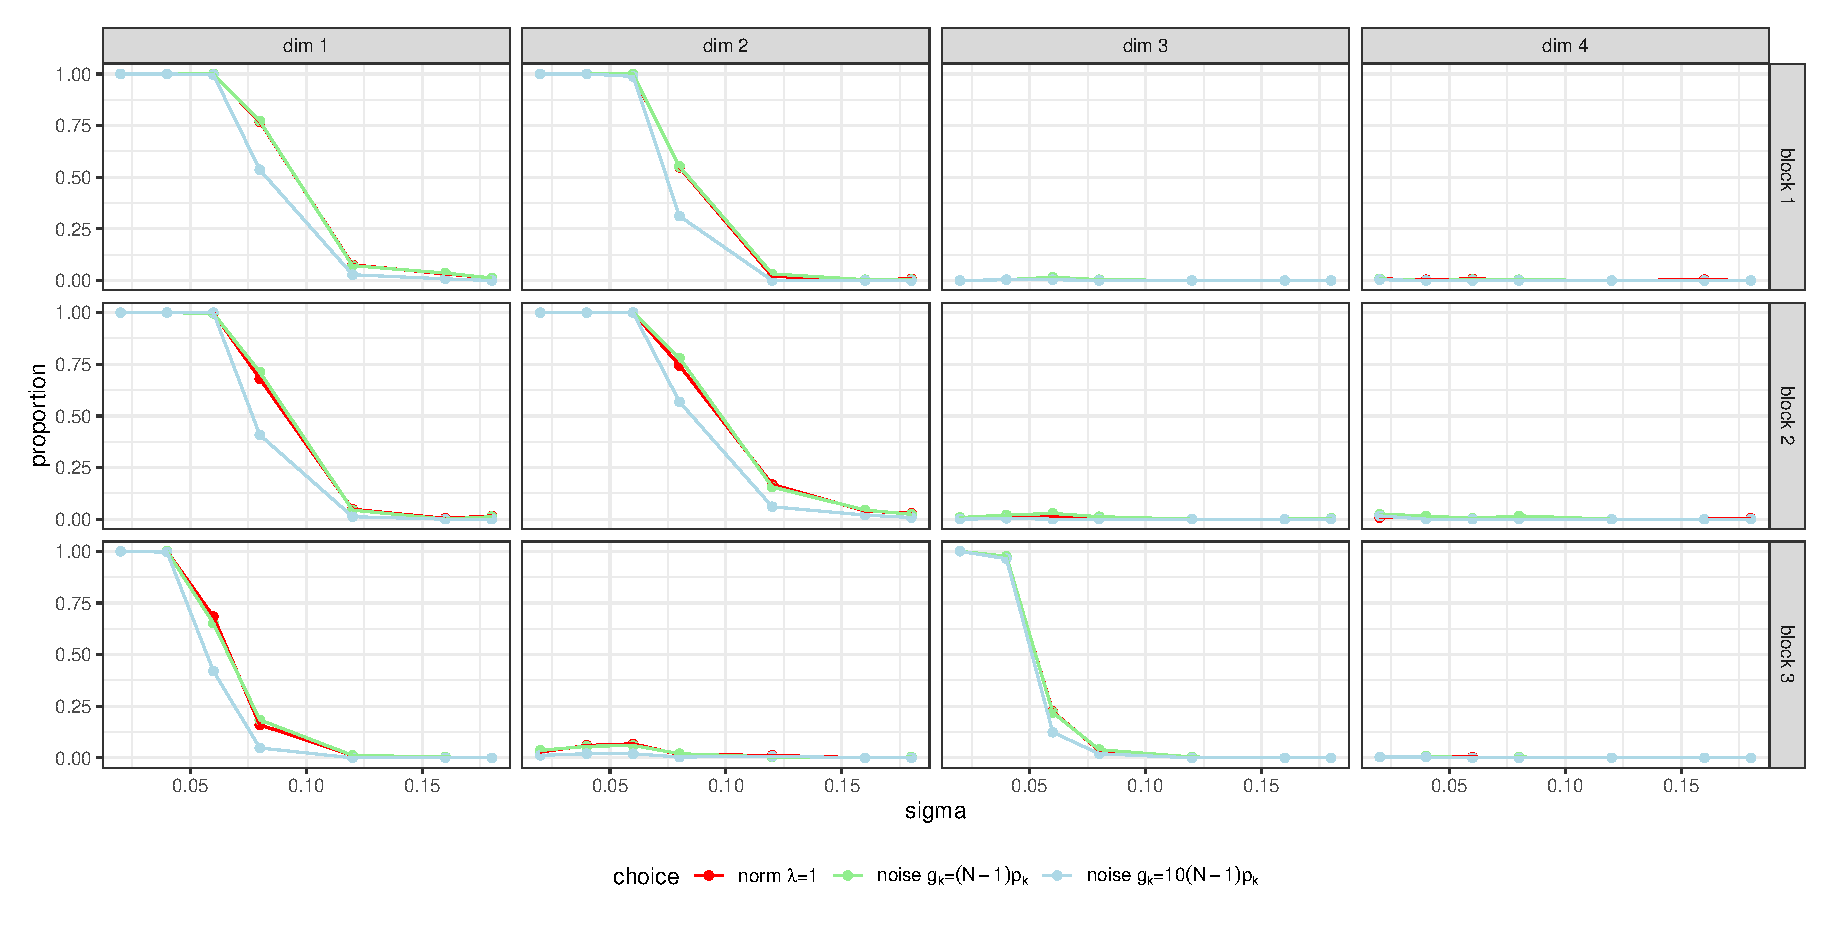
\includegraphics[width=\linewidth]{figs/choice_l_vs_g.eps}
  \caption{Empirical probability that a dimension is selected in a block, as a function of the noise standard deviation $s$, for the slab scaled by the block norm ($\lambda=1$, red) and the slab indexed on the noise with $g_k=(N-1)p_k$ (green) and $g_k=10(N-1)p_k$ (blue).  \label{fig:choice_l_vs_g}}
\end{figure}

\paragraph{Spike parameter:} Figure~\ref{fig:choice_spike} illustrates the probability that a dimension will be selected based on the spike parameters $(a_\theta,b_\theta)$, using the default value for $\lambda$ ($\lambda=1$). The three priors gave similar results in all the blocks, and none of them selected the zero weights: the selection is driven by the data rather than by the prior distribution of $\Reff$, although these priors differ markedly (Table~\ref{tab:spike_param}). The most conservative prior $(1,3)$ lost the active weights at slightly lower noise levels (dimension 1 in blocks 1 and 3, $s=0.06$--$0.08$). The probability of including dimension 3 in block 3 was the same for the three priors: this dimension is only present in block 3, so that $\theta_3$ is informed by this block alone, and its inclusion probability dropped sharply from $s=0.06$ to $s=0.08$ whatever the prior, even with the prior that favours the true rank. For dimension 1 in block 3, the inclusion probability decreased slightly less with the all-or-nothing prior $(0.5,0.5)$, since dimension 1 is selected in blocks 1 and 2 and the stronger coupling transfers this information to block 3. In the following, the spike parameters are set to their default value $(1,1)$.    

\begin{figure}
  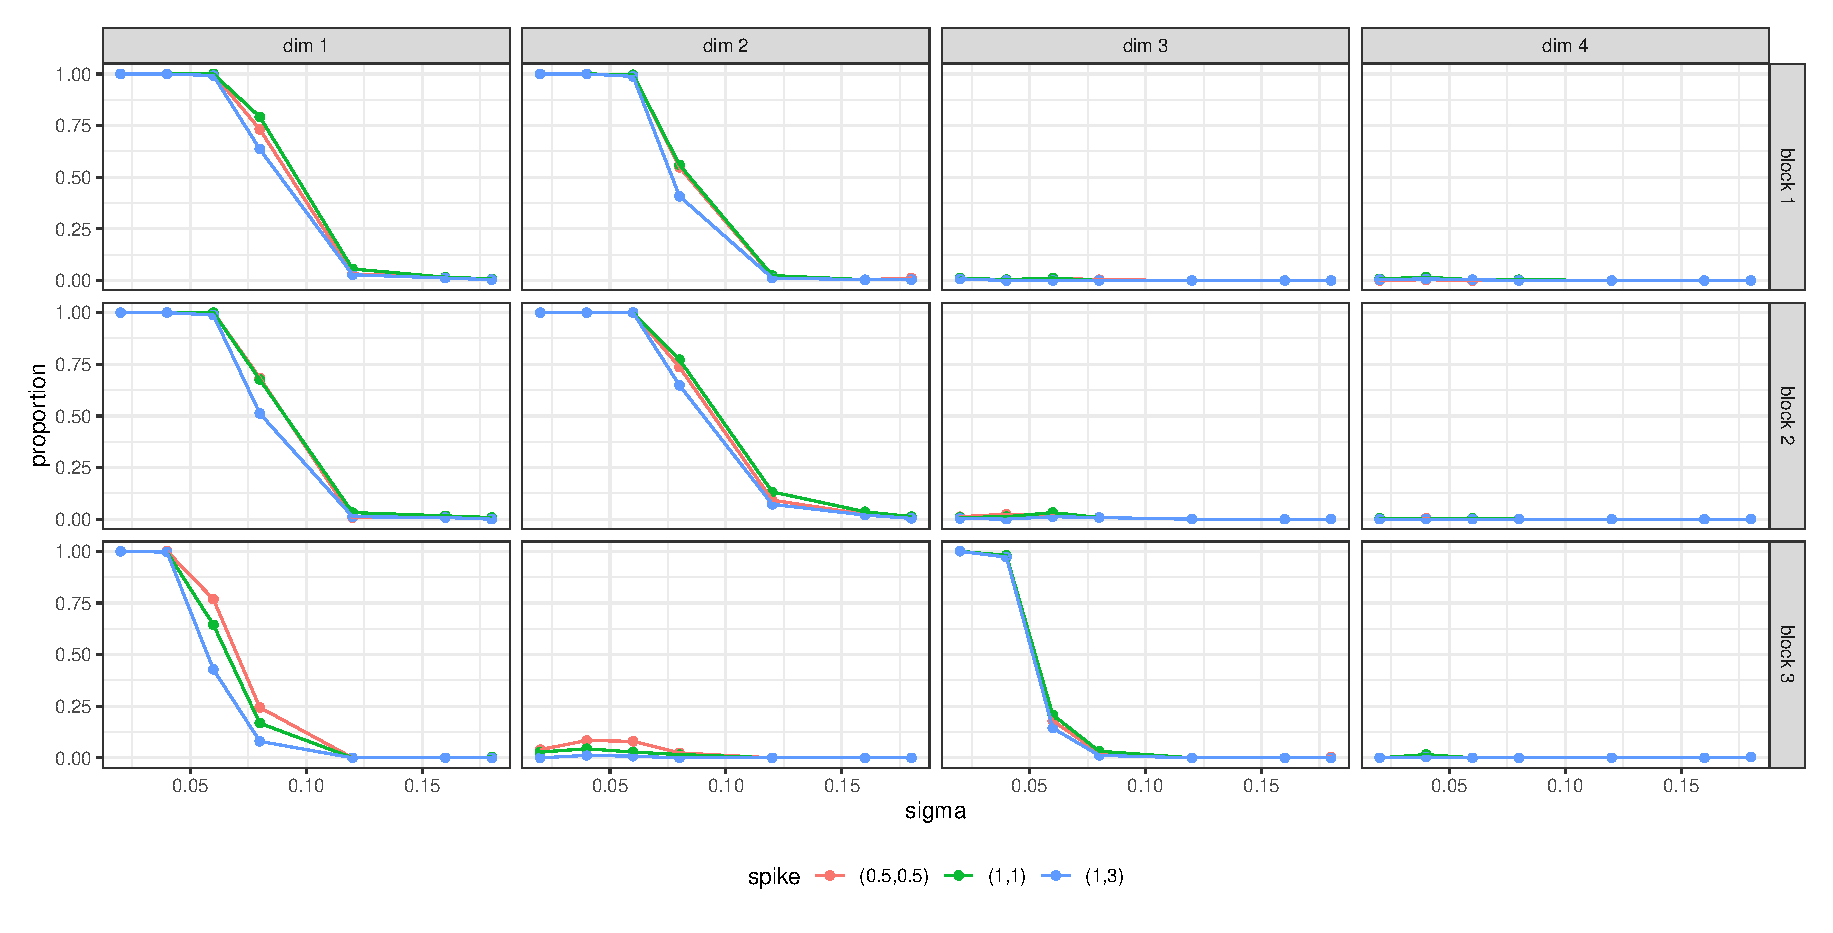
\includegraphics[width=\linewidth]{figs/choice_spike.eps}
  \caption{Empirical probability that a dimension is selected in a block, as a function of the noise standard deviation $s$ and of the spike parameter $(a_\theta,b_\theta)$ (red for $(0.5,0.5)$, green for $(1,1)$ and blue for $(1,3)$). \label{fig:choice_spike}}
\end{figure}

\paragraph{Slab parameter:} Figure~\ref{fig:choice_lambda} provides the probability of selection of a dimension $r$ on a block $k$ as a function of the noise parameter $s$ and the slab precision $\lambda$. For all $\lambda$, when the noise standard deviation was low ($s<0.06$), all the active dimensions were selected. When $s$ increased ($s>0.08$), the active weights were lost in the following order: dimension 3 on block 3 , dimension 1 on block 3, dimension 2 on block 1, dimension 1 on block 2, dimension 1 on block 1, and finally dimension 2 on block 2. Apart from the first two, this order followed the detectability thresholds of Table~\ref{tab:thres}. The first two were inverted: the weight $0.3$ of dimension 1 on block 3 (threshold $0.05$) was still selected in about 65\% of the data sets for $s=0.06$ ($\lambda=1$), whereas the weight $0.5$ of dimension 3 on block 3 (threshold $0.08$) was already selected in only about 25\% of them. Dimension 1 is shared by the three blocks, so that $\uu^{(1)}$ is well estimated from blocks 1 and 2 and its weight in block 3 remains detectable beyond the single-block threshold. Dimension 3 is only present in block 3: $\uu^{(3)}$ is estimated from this block alone, and the Bayes factor requires a margin above the spectral threshold. The multiblock model therefore borrows strength across blocks and detects weights that a block-by-block analysis would miss.
With the two more conservative values $\lambda=0.1$ and $\lambda=1$, dimension 4 , as well as the zero weights of dimensions 1 to 3 (dimension 3 on blocks 1 and 2, dimension 2 on block 3), were almost never selected. With $\lambda=10$, the active weights were lost at slightly higher noise levels, at the cost of about 25\% of false selections in blocks 1 and 2 and more than 75\% of false selections in block 3. In this design, $\lambda=1$ offered the best trade-off between the detection of weak weights and false selections.    

\begin{figure}
  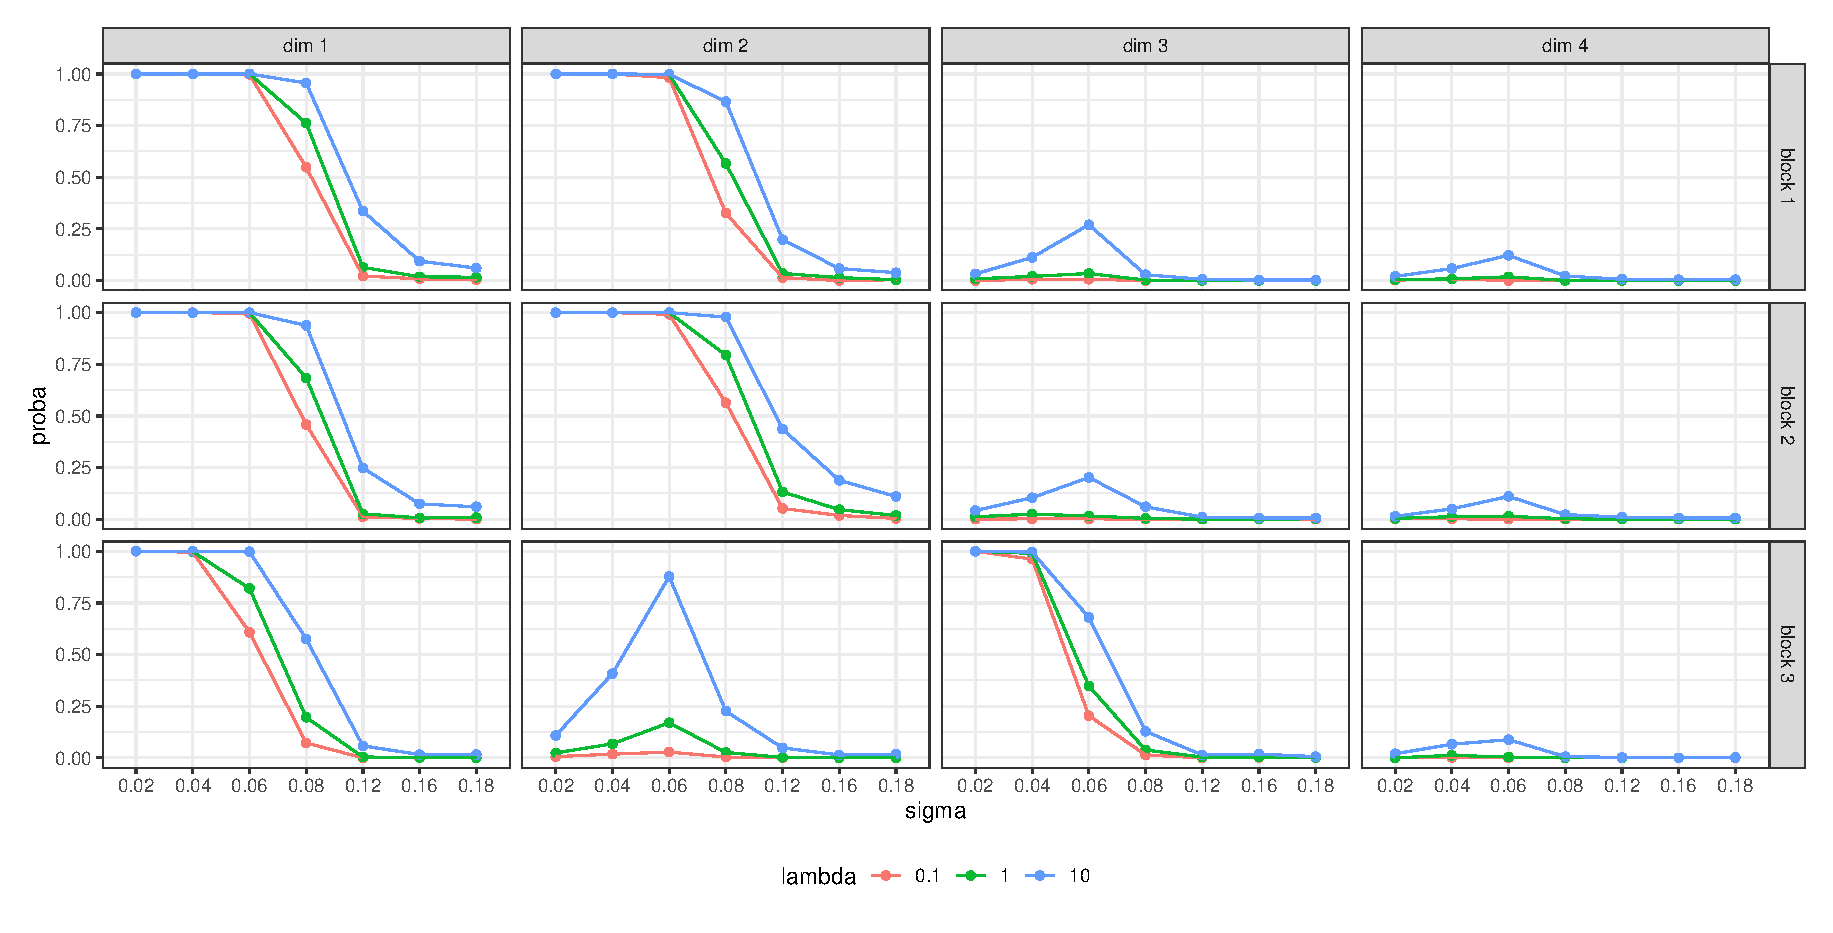
\includegraphics[width=\linewidth]{figs/choice_lambda.eps}
  \caption{Empirical probability that a dimension is selected in a block, as a function of the noise standard deviation $s$ and of the slab precision $\lambda$. \label{fig:choice_lambda}}
\end{figure}

\subsubsection*{MCMC diagnostics:} Table~\ref{tab:mcmc_diag} presents the MCMC diagnostics of the sparse Gibbs sampler for one simulated data set per noise level $s$, computed with the rank-normalised $\hat R$ and bulk effective sample sizes of \citet{vehtari2021}, on the aligned draws for the weights. Four chains were run: two with all the indicators $\gamma_k^{(r)}$ initialized to 0, and two with all of them initialized to 1. The chains consisted of $T=6000$ iterations with a burn-in of $T_0=2000$. Far from the detectability thresholds ($s=0.04$ and $s=0.12$), the chains mixed well and the effective sample sizes were large for all the parameters. Close to the thresholds ($s=0.06$ and $s=0.08$), the chains started from $\gamma=0$ and from $\gamma=1$ reached the same posterior distribution of $\Reff$ ($\hat R\leq1.01$, largest difference of the posterior probabilities between chains $\leq0.11$; see Figures~\ref{fig:diag1} and~\ref{fig:diag2} in Appendix~\ref{sec:mcmc_diag}), but the mixing was slower, with a bulk effective sample size of 175 for $\Reff$ at $s=0.08$. The smallest effective sample size (70, $s=0.06$) concerned the weight of dimension 2 in block 3, which is truly zero: its draws are 0 except during rare excursions in the slab, which inflates their autocorrelation without affecting the posterior inclusion probability.  
\begin{table}[ht]
\centering
\begin{tabular}{rrrrrrrrrr}
  \hline
$s$ & $\hat R(\Reff)$ & $\max(D_{\Reff})$ & $bulkESS(\Reff)$ & $\max(\hat R(\sigma^{(r)}_k))$ &  $k_1$ & $r_1$ & $\min(bulkESS(\sigma^{(r)}_k))$ & $k_2$ & $r_2$ \\ 
  \hline
0.04 & 1.01 & 0.10 & 596.00 & 1.01 &   2 &   4 & 420.00 &   3 &   4 \\ 
  0.06 & 1.00 & 0.05 & 750.00 & 1.05 &   3 &   2 & 70.00 &   3 &   2 \\ 
  0.08 & 1.01 & 0.11 & 175.00 & 1.03 &   2 &   3 & 115.00 &   2 &   3 \\ 
  0.12 & 1.01 & 0.06 & 473.00 & 1.01 &   2 &   4 & 341.00 &   2 &   4 \\ 
   \hline
\end{tabular}
\caption{MCMC diagnostics for the weights and the effective rank as a function of the noise standard deviation $s$ (four chains, one simulated data set per value of $s$). $\max(D_{\Reff})$ denotes the maximum difference in $\Reff$ between the four chains, $bulkESS$ denotes the bulk effective sample size, $(k_1,r_1)$ designates the couple of the block/dimension corresponding to $\max(\hat R(\sigma^{(r)}_k))$ and $(k_2,r_2)$ designates the couple of the block/dimension corresponding to $\min(bulkESS(\sigma^{(r)}_k))$. \label{tab:mcmc_diag}}
\end{table}


\subsubsection*{Estimation of the weights $\sigma_k^{(r)}$:}
Figure~\ref{fig1} provides the empirical coverage of the 95\% credible intervals of the block weights of dimensions 1 to 3, as a function of the noise standard deviation $s$, for the non-sparse sampler and the sparse sampler with $\lambda=1$. The coverage was close to the nominal level for $s\leq0.04$. For the weights equal to zero, the coverage of the non-sparse sampler was 0, since its half-normal prior excludes the value 0, whereas the sparse sampler covered the true value in all cases. For the active weights at high noise levels, the non-sparse sampler was over-conservative, with a coverage close to 1, since its credible intervals widened. For the active weights, the coverage of the sparse sampler first decreased when $s$ increased, the weight of dimension 3 in block 3, which is only present in this block, being the first affected (coverage of about 0.5 at $s=0.08$). Near the thresholds, the posterior distribution of the weight mixes the spike at 0 and a slab component that underestimates the weight, so that the credible interval may miss the true value. At higher noise levels, the coverage increased again, although the weights were rarely selected (Figure~\ref{fig:choice_lambda}): as long as $P(\gamma_k^{(r)}=1\mid\X)$ is not negligible, the credible interval is of the form $[0,q_{0.975}]$, and the slab draws, which are diffuse when the signal is weak, make it wide enough to contain the true value. The interval is reduced to $\{0\}$ only when $P(\gamma_k^{(r)}=1\mid\X)<0.025$. For $s\geq 0.12$, the coverage is  not informative since the width of the intervals are very large (in mean greater than 0.90 for Gibbs sampler of OMCOA and in mean greater than 0.53 for Gibbs sampler of sparse OMCOA). Figure~\ref{fig2} provides the estimated block weights of the active dimensions, with the 2.5\% and 97.5\% empirical quantiles over the $B$ replications, as a function of $s$. When the weights were nonzero, they were accurately estimated by the two Bayesian samplers and by MCOA and OMCOA for $s\leq0.04$. The upward bias of MCOA and OMCOA increased with $s$, since these methods fit part of the noise, which inflates the estimated weights. The non-sparse Gibbs sampler degraded less. The sparse sampler behaved differently: a weight that is not detected is set to 0, so that the true zero weights were kept at 0, whereas the active weights were biased downwards at high noise levels; for instance, the weight $0.7$ of dimension 1 on block 1 was estimated between about $0.1$ and $0.3$ for $s\geq0.12$. This is a consequence of the selection, not an absence of bias.

\begin{figure}
  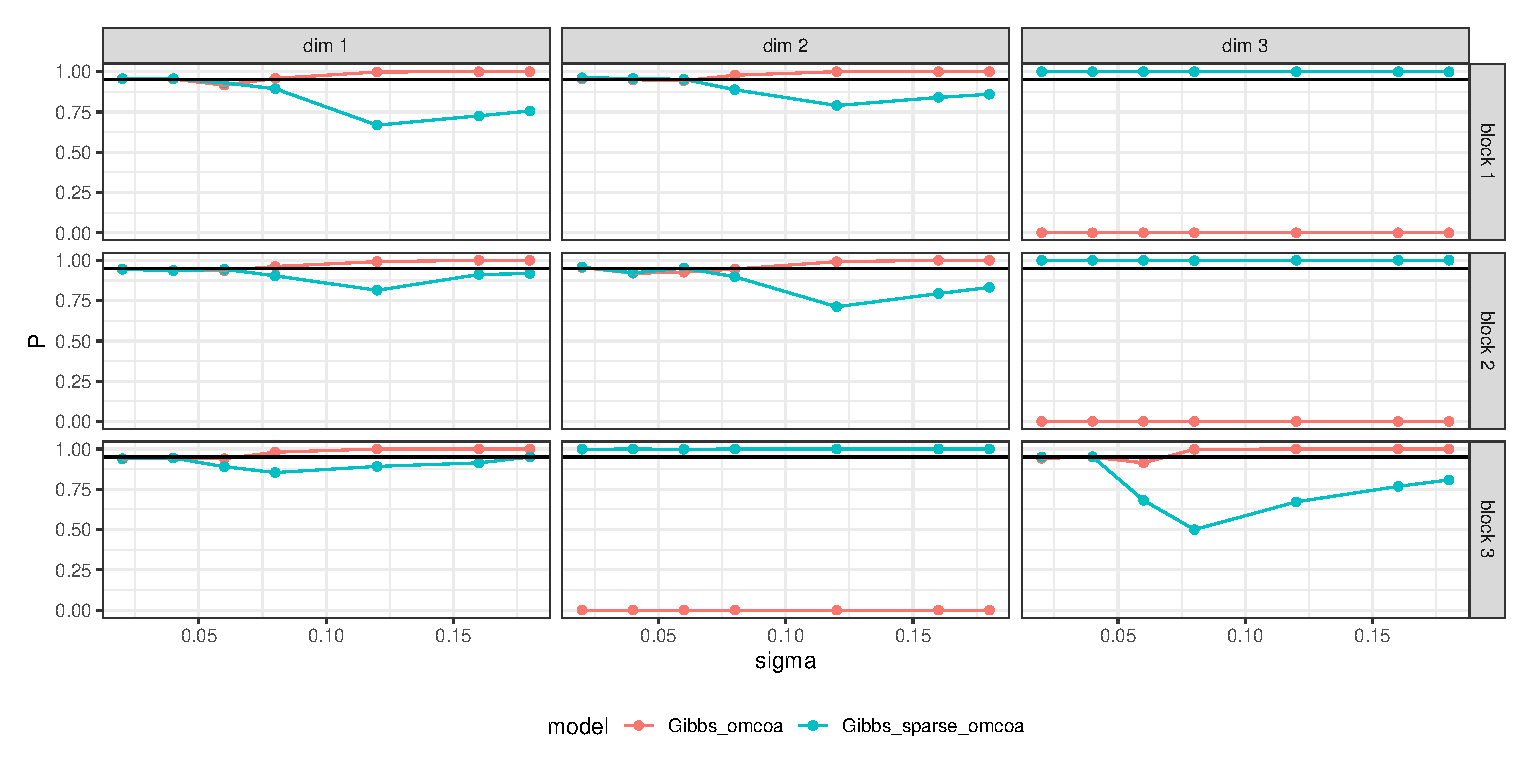
\includegraphics[width=\linewidth]{figs/cov_percent.eps}
  \caption{Empirical coverage probability of the weights $\sigma_k^{(r)}$ using Gibbs sampler for OMCOA (in red), Gibbs sampler for sparse,OMCOA with $\lambda=1$ (in blue) as a function of the noise standard deviation $s$. \label{fig1}}
\end{figure}



\begin{figure}
  \centering
  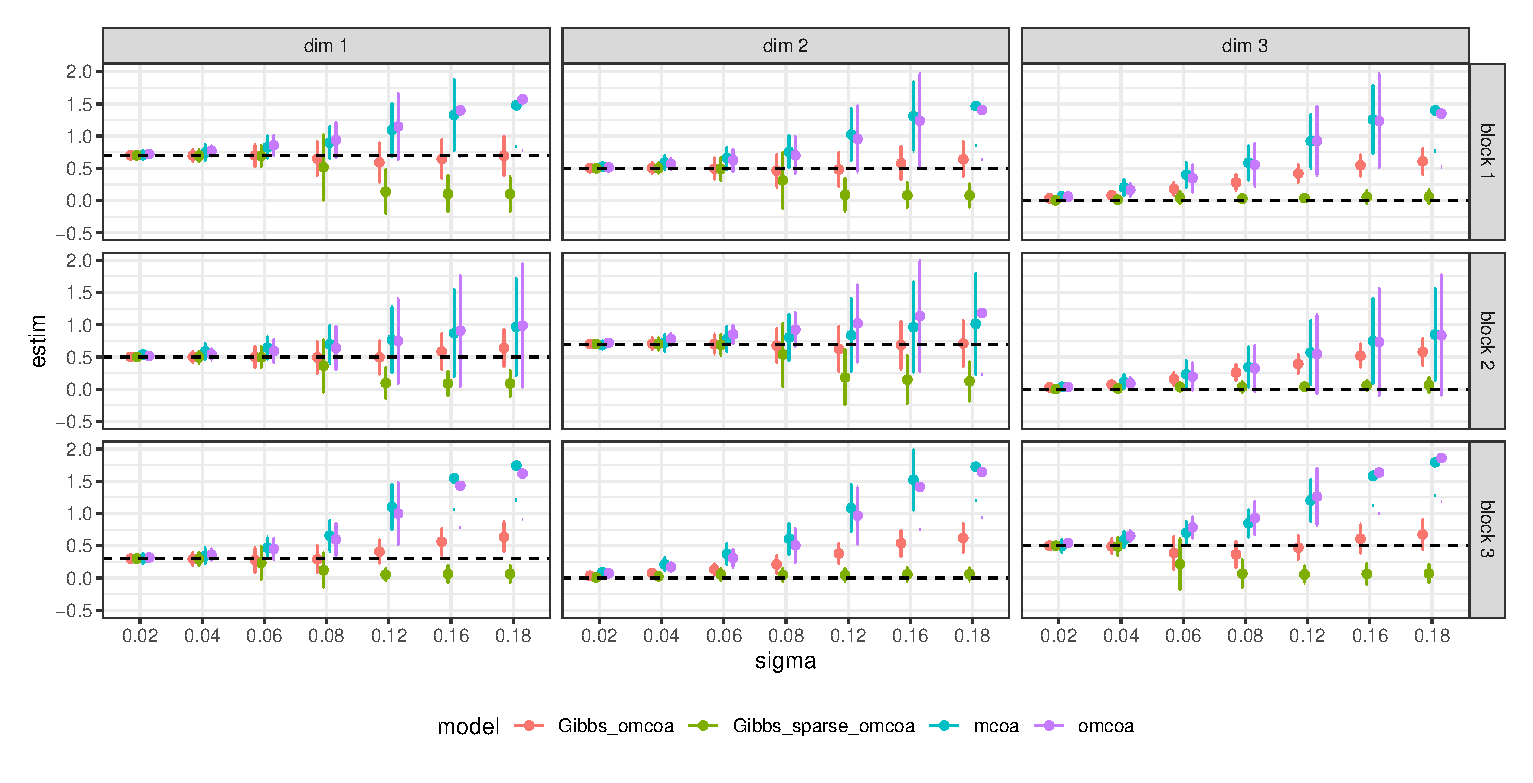
\includegraphics[width=\linewidth]{figs/bias_estimation.eps}
  \caption{Estimated block weights, with the 2.5\% and 97.5\% empirical quantiles over the $B=1000$ simulated data sets, for dimensions 1 to 3 (the dashed lines give the true values, including the zero weights), obtained using the sequential approach (MCOA in blue), the simultaneous approach (OMCOA in purple), the Gibbs sampler for OMCOA (Gibbs sampler for OMCOA in red) and the sparse version (Gibbs sampler for sparse OMCOA with $\lambda=1$ in green), as a function of the noise standard deviation $s$. For Bayesian models, the estimate is equal to the posterior mean.  \label{fig2}}
\end{figure}
For the inactive dimension 4 (not shown), the estimated weights of MCOA, OMCOA and of the non-sparse sampler increased with $s$, since these methods fit the noise, whereas the sparse sampler kept them at 0 in almost all cases.



\subsubsection*{Comparison of the estimates of the effective rank:} Figure~\ref{fig6} provides the distribution of the estimated effective rank over the $B$ simulated data sets as a function of the noise standard deviation $s$, for the Gavish--Donoho threshold, the sparse Gibbs sampler and Hoff's Bayesian SVD. For $s=0.02$, the three methods recovered the true rank $\Reff=3$ in all the data sets. The Gavish--Donoho threshold was the first to underestimate the rank: it selected 2 dimensions in almost all the data sets from $s=0.04$, and 1 dimension in about 70\% of them for $s\geq0.12$. The sparse Gibbs sampler recovered $\Reff=3$ in almost all the data sets for $s\leq0.04$ (with a few cases of $\Reff=4$) and in about 75\% of them for $s=0.06$; for $s=0.08$, it mostly selected 2 dimensions (about 70\% of the data sets), after losing dimension 3, which is only present in block 3 (Figure~\ref{fig:choice_lambda}). This underestimation occurred although the default prior favours $\Reff=3$ or 4 (Table~\ref{tab:spike_param}): it is driven by the data. Hoff's Bayesian SVD performed better in this intermediate range: it recovered $\Reff=3$ in all the data sets for $s=0.06$ and in about 75\% of them for $s=0.08$. Hoff's method only estimates the rank of the concatenated matrix: it does not indicate in which blocks a dimension is active, which is the purpose of the sparse model. Moreover, a dimension carried by a single block is selected by the sparse model through the Bayes factor of this block alone, which requires a margin above the single-block detectability threshold (Section~5.2), whereas it contributes to a singular value of the concatenated block in Hoff's model. At high noise levels ($s\geq0.12$), the behaviours were reversed: Hoff's Bayesian SVD estimated $\Reff=0$ in most of the data sets (about 90\% for $s=0.18$), whereas the sparse sampler mostly kept $\Reff=1$ (between 55\% and 70\% of the data sets), i.e.\ dimension 1, which is shared by the three blocks. This is the borrowing of strength across blocks observed in Figure~\ref{fig:choice_lambda}: a dimension that is weak in each block but common to all of them remains detectable.   

\begin{figure}
  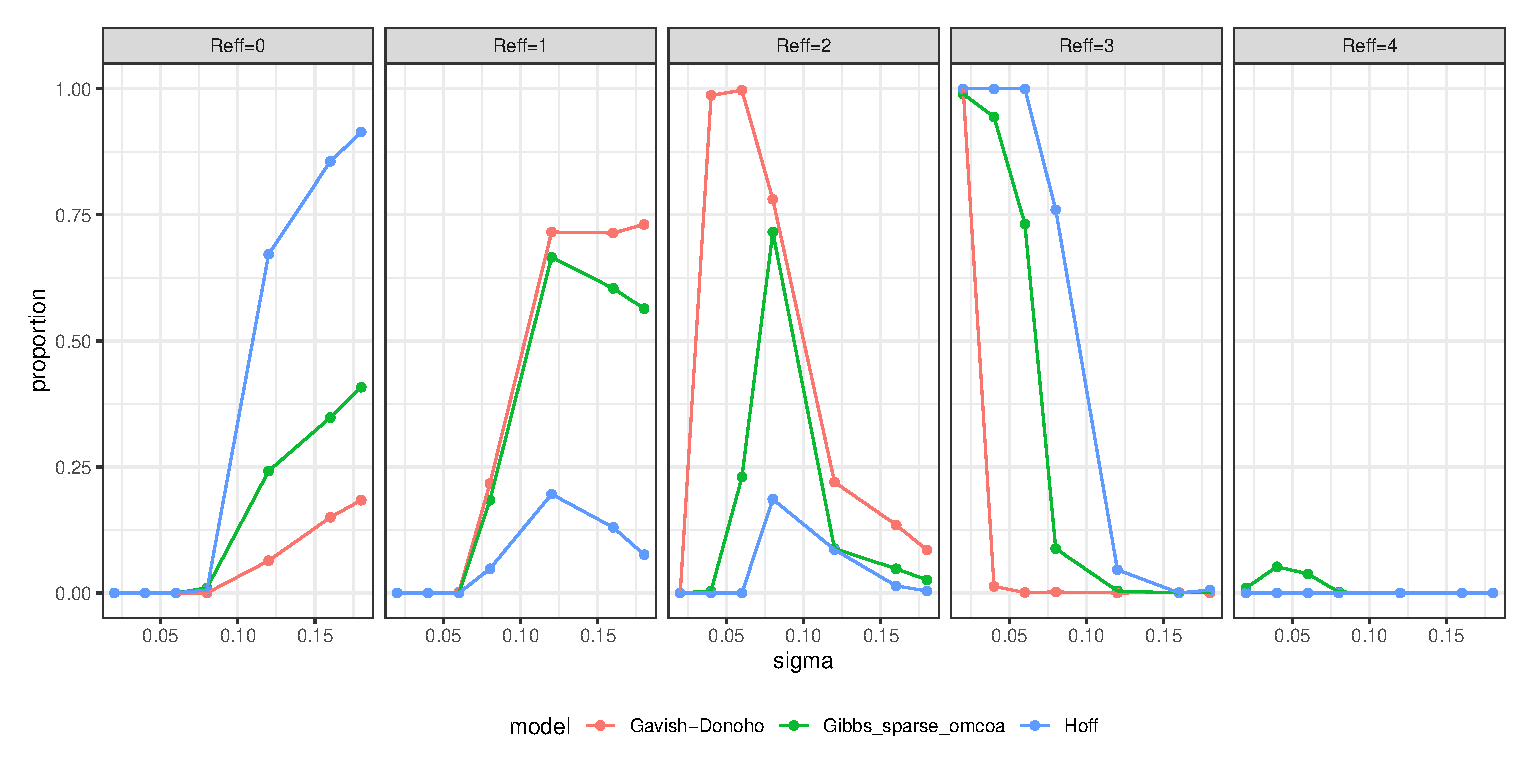
\includegraphics[width=\linewidth]{figs/Reff_comparison.eps}
  \caption{Distribution of the estimated effective rank over the $B$ simulated data sets for the Gavish--Donoho threshold, the sparse Gibbs sampler ($\lambda=1$, $a_\theta=b_\theta=1$) and Hoff's Bayesian SVD, as a function of the noise standard deviation $s$ (true value $\Reff=3$). \label{fig6}}
\end{figure}

\section{Application to breast cancer multi-omics data}\label{sec:appli}
 
\paragraph{Data.} We use the \texttt{breast.TCGA} data of the \textsf{R} package \texttt{mixOmics} \citep{rohart2017}, a subset of The Cancer Genome Atlas breast cancer data \citep{tcga2012} used to illustrate multiblock methods \citep{singh2019}. The training set contains $N=150$ tumours described by $K=3$ blocks: the expression of $p_1=184$ microRNAs, of $p_2=200$ genes (mRNA) and the abundance of $p_3=142$ proteins. The PAM50 subtype of the tumours (Basal, $n=45$; Her2, $n=30$; Luminal A, $n=75$) is not used in the fit, only for the interpretation. The variables were only centred: the samplers are invariant to the scale of the blocks, and a block normalisation is not needed (Section~4). The sparse Gibbs sampler was run with $\lambda=1$, $a_\theta=b_\theta=1$ and $R_{\max}=40$, with four chains of $T=6000$ iterations (burn-in $T_0=2000$, thinning 10), two started with all the indicators equal to 1 and two with all of them equal to 0.
 
\paragraph{Dominant dimensions.} The leading dimensions were selected with a posterior probability equal to 1 in all the chains, and their weights were estimated with narrow credible intervals (Figure~\ref{fig:tcga_weights}). The first dimension is common to the three blocks: it explains about 17\%, 20\% and 21\% of the variance of the miRNA, mRNA and protein blocks, respectively ($(\sigma_k^{(1)}/\|\X_k\|)^2$). It is followed by a few strong dimensions which are mainly specific to one block, for instance a dimension which explains about 11\% of the variance of the mRNA block and 6\% of the miRNA block but is almost absent from the protein block, and a dimension specific to the protein block (about 12\% of its variance). Beyond these, a long series of dimensions explains less than 2--3\% of the variance of each block. The two dimensions most associated with the subtype are both active in the three blocks, with a posterior inclusion probability equal to 1 in each block and in each of the four chains, whatever their initialisation. The posterior means of the $R^2$ of the regression of their components on the subtype are $0.89$ (95\% credible interval $[0.885,0.898]$) and $0.61$ ($[0.58,0.65]$). Their components separate the three subtypes (Figure~\ref{fig:tcga_subtype}): the first one, which is the common dimension described above, opposes the Basal and Luminal A tumours, and the second one isolates the Her2 tumours. 
The loadings of the first dimension are consistent with the biology of the subtypes. 
The component of the first dimension being positive for the Luminal A tumours and negative for the Basal tumours, the variables with large positive loadings are more expressed in the Luminal A tumours: the hormone receptors ER-$\alpha$ and PR and the transcription factor GATA3 among the proteins (loadings 0.55, 0.41 and 0.28), and oestrogen-regulated genes such as STC2, NTN4 and ZNF552 among the mRNAs. Conversely, the proliferation markers Cyclin B1 (protein), ASPM and CCNA2 (mRNA) have negative loadings, as do almost all the miRNAs with the largest loadings, which are therefore more expressed in the Basal tumours: miR-9 (both precursors), the miR-17-92 family (miR-17, miR-20a, miR-106a), miR-146a and the hypoxia-induced miR-210. The second dimension is driven by the Her2 tumours, whose component is negative while it is positive for both the Basal and the Luminal A tumours. The proteins with the largest negative loadings, i.e.\ more abundant in the Her2 tumours, are HER2 itself ($-0.41$) and its phosphorylated form HER2\_pY1248 ($-0.33$), together with the phosphorylated EGFR ($-0.26$) of the same receptor family and the androgen receptor AR ($-0.22$), whereas the progesterone receptor PR has a positive loading ($0.30$), in agreement with the hormone receptor negative status of most HER2-enriched tumours. Among the miRNAs, miR-30a and miR-181c/d have positive loadings, i.e.\ are less expressed in the Her2 tumours. The mRNA block contributes less specifically to this dimension, its largest loadings being positive (STC2, NDRG2, CDK18). Since the positive side of this component gathers two subtypes, its positive loadings indicate a lower expression in the Her2 tumours rather than a marker of a given subtype. Thus, two dimensions shared by the three blocks, identified without using the subtype, recover the PAM50 classification.
 
\paragraph{Effective rank.} In contrast, the effective rank was not identified. In the chains started with all the dimensions active, $\Reff$ remained equal to $R_{\max}=40$; in the chains started with all of them inactive, it started at about 25 and was still slowly increasing at the end of the run (Figure~\ref{fig:tcga_diag}). The noise precisions of the two groups of chains also differed (e.g.\ $\tau_3\approx8.0$ versus $7.1$), the chains started from $\gamma=0$ moving slowly towards the others. The weak dimensions therefore mix very slowly, as anticipated in Section~4, and their inclusion probabilities averaged over the chains are not reliable. This saturation is consistent with short runs of the sampler for $R_{\max}=10$, $20$ and $40$, for which $P(\Reff=R_{\max}\mid\X)\approx1$, and with the Gavish--Donoho threshold, which retains 30, 19 and 28 dimensions for the miRNA, mRNA and protein blocks separately.
 
Additional experiments (Appendix~\ref{sec:saturation}) point to a misspecification of the noise rather than to a failure of the sampler. With blocks of the same dimensions made of i.i.d.\ Gaussian noise, the sampler returned $\Reff\approx0$--$1$ from both initialisations. With blocks made of independent columns having the standard deviations of the TCGA variables, which range from 0.2 to 2.5 within a block, but no common structure, it reproduced the behaviour observed on the real data: saturation at $R_{\max}$ from the chains started with all the dimensions active, and a slow increase from the others. Since the model assumes a common noise variance within each block, the variables with a large variance are explained by additional dimensions. Standardising the variables did not remove the saturation on the real data, since their spectrum decreases slowly without a clear gap between signal and noise: with $N=150$ tumours, many weak but genuine correlations are detectable.
 
On such data, $\Reff$ measures the departure from the low-rank plus white noise model rather than a number of latent factors, and it grows with $R_{\max}$ and $N$. The dominant dimensions, their pattern of activity across the blocks and their explained variances remain interpretable and stable across the chains. A natural extension is a noise precision per variable, $\tau_{kj}$; the full conditionals of the loadings $\V_k$ are then matrix Bingham--von Mises--Fisher distributions, which can be simulated with the algorithm of \citet{hoff2009}.
 
\begin{figure}
  \centering
  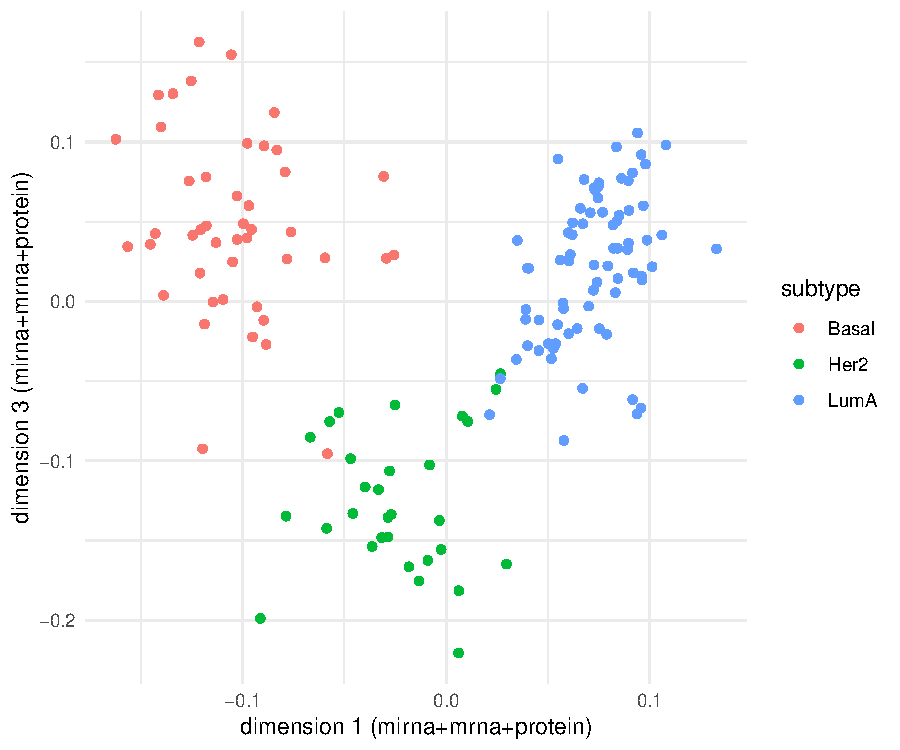
\includegraphics[width=0.6\linewidth]{figs/components_subtype.pdf}
  \caption{Breast cancer data: posterior means of the two components most associated with the PAM50 subtype, both active in the three blocks, coloured by subtype. \label{fig:tcga_subtype}}
\end{figure}
 
\begin{figure}
  \centering
  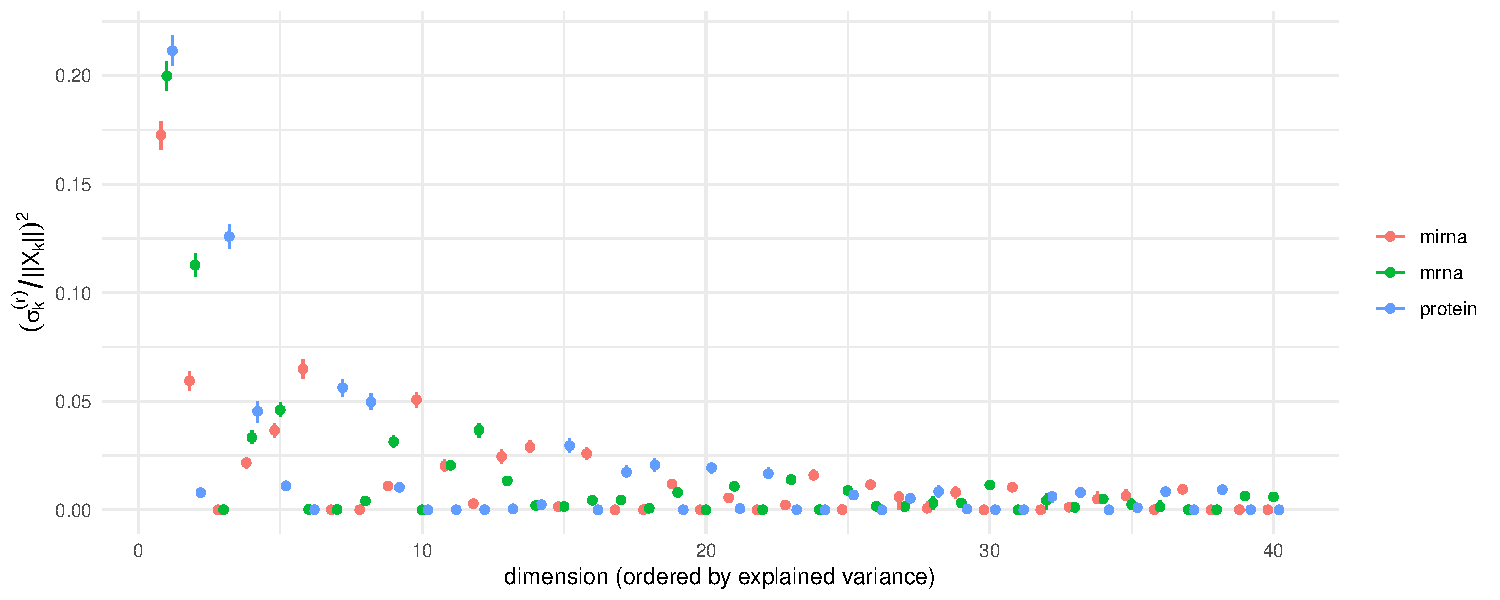
\includegraphics[width=\linewidth]{figs/weights_all.pdf}
  \caption{Breast cancer data: posterior means and 95\% credible intervals of the proportions of variance $(\sigma_k^{(r)}/\|\X_k\|)^2$ explained by each dimension in each block, the dimensions being ordered by total explained variance. Draws of the two chains started with all the dimensions active ($\gamma_k^{(r)}=1$); the chains started with $\gamma_k^{(r)}=0$ give the same weights for the leading dimensions (Appendix~\ref{sec:saturation}). \label{fig:tcga_weights}}
\end{figure}

\section{Discussion}\label{sec:discussion}
 
We have proposed a Bayesian formulation of the canonical factorization of multiblock data with orthonormal block loadings, whose posterior mode is computed by the OMCOA algorithm, and a sparse version which selects, for each dimension, the blocks in which it is active. The orthonormality of the loadings gives full conditional distributions of the matrix von Mises--Fisher type, which can be simulated exactly column by column, and the spike-and-slab prior on the block weights has a closed-form Bayes factor. The model is identified as soon as the profiles of the block weights of the dimensions are distinct, a weaker condition than that of MCOA, whose dimensions are only identified by weighted sums of the squared block weights (Proposition~\ref{prop:identif}). With a slab scaled by the norm of each block and the Jeffreys prior on the noise precisions, the posterior distribution of the components, of the loadings and of the indicators does not depend on the scale of the blocks, so that no block weighting or standardisation has to be chosen. The slab indexed on the noise level, in the spirit of Zellner's $g$-prior, gave almost the same selection.
 
The posterior distribution of the indicators $\gamma_k^{(r)}$ provides, beyond an estimate of the effective rank $\Reff$, the pattern of activity of each dimension across the blocks, with its uncertainty. In the simulations, the selection was driven by the data rather than by the prior: the three priors on the inclusion probabilities, which imply very different prior distributions of $\Reff$, gave similar selection probabilities, and the weights were lost in the order predicted by the single-block detectability thresholds. Since the inclusion probability $\theta_r$ of a dimension is shared by the blocks, a dimension which is weak in each block but common to all of them remained detectable beyond these thresholds, whereas Hoff's Bayesian SVD of the concatenated matrix then estimated an effective rank of zero in most data sets. Conversely, a dimension carried by a single block is selected from the evidence of this block alone, and was lost at lower noise levels than with Hoff's Bayesian SVD, which only estimates the rank of the concatenated matrix and does not indicate which blocks carry each dimension.
 
On the breast cancer data, the dimensions with the largest weights were selected with probability one in all the chains, and the two dimensions shared by the three blocks that are most associated with the PAM50 subtype recovered the classification of the tumours, with loadings consistent with the known biology of the subtypes. The effective rank was not identified, however: it reached the maximal rank, and the weak dimensions mixed very slowly. Our experiments relate this behaviour to the noise model rather than to the sampler: a common noise variance within each block cannot account for variables whose variances differ by an order of magnitude, and the spectrum of these data has no clear gap between signal and noise. This points to the main limitations of the approach, and to several extensions.
 
\paragraph{Noise model.} The assumption of an i.i.d.\ Gaussian noise within each block is the main limitation for omics data. A noise precision $\tau_{kj}$ per variable keeps the conjugacy of the noise precisions, but the full conditional distribution of the loadings $\V_k$ then becomes a matrix Bingham--von Mises--Fisher distribution, which can still be simulated with the algorithm of \citet{hoff2009}. This extension would also make the comparison with methods which standardise the variables more meaningful. Heavier-tailed noise distributions could be introduced through scale mixtures of normals, at the price of one additional latent variable per entry.
 
\paragraph{Mixing of the indicators.} The indicators are drawn with the block weights integrated out, but given the loadings. When a dimension is inactive, its loadings are uniform, and the dimension can be reactivated only when a uniform draw happens to align with the signal, which is slow in high dimension; conversely, an active dimension whose loadings are aligned with the data is rarely deactivated. Both effects were visible on the real data. A move which updates jointly $\gamma_k^{(r)}$, $\sigma_k^{(r)}$ and $\vv_k^{(r)}$, with the loadings integrated out through the normalising constant of the von Mises--Fisher distribution, or tempering strategies, should improve the mixing. In the meantime, we recommend running chains started with all the dimensions active and with none of them, as done here.
 
\paragraph{Prior on the effective rank.} With independent Beta priors on the inclusion probabilities, the prior expectation of $\Reff$ grows linearly with the maximal rank $R_{\max}$. The prior $\theta_r\sim\Be(\alpha/R_{\max},1)$ of Section~4 makes it nearly independent of $R_{\max}$; a nonparametric version, with an unbounded number of dimensions as in the Indian buffet process \citep{griffiths2011} or with increasing shrinkage of the successive dimensions \citep{bhattacharya2011,legramanti2020}, would remove the choice of $R_{\max}$ altogether, at the cost of an adaptive sampler.
 
\paragraph{Other extensions.} The Bayesian formulation handles missing entries, or missing blocks for some observations, by data augmentation, as in the Bayesian SVD of \citet{zhai2023}; this is the case of the test set of the breast cancer data, which has no protein block. The computational cost of an iteration grows linearly with $R_{\max}$ and with the total number of variables, and was of the order of a few tenths of a second for $R_{\max}=40$ on the breast cancer data; for much larger data sets, a variational approximation of the posterior distribution would be a natural complement, the Gibbs sampler providing a reference to assess it.
 
\paragraph{Conclusion.} The sparse Bayesian OMCOA turns the choice of the number of dimensions of a multiblock factorization into a posterior inference on which dimensions are active in which blocks. It is invariant to the scale of the blocks, borrows strength across blocks for the dimensions they share, and provides credible intervals for the block weights and posterior probabilities for the effective rank. On real data, the inference on the dominant dimensions was stable and interpretable, while the inference on the effective rank requires a noise model adapted to the data. The methods are implemented in the \textsf{R} package  \href{https://github.com/GALHARRET/BayesCanoFacto}{\texttt{BayesCanoFacto}} available on GitHub.



\clearpage



\bibliographystyle{apalike}
\bibliography{Biblio}


\appendix
\section{Proofs of the propositions}

\begin{proof}[Proposition 1]
	The criterion to be minimized is:
\[
  \mathcal{L}(\U, \V_1, \ldots, \V_K, \Sigma_1, \ldots, \Sigma_K)
  = \sum_{k=1}^{K} \bigl\| \X_k - \U \Sigma_k \V_k^\top \bigr\|^2,
\]
subject to $\U\in\Stiefel{N}{R}$ and $\V_k\in \Stiefel{p_k}{R}$ for all $k = 1, \ldots, K$.

The algorithm is of the \emph{Alternating Least Squares} (ALS) type: at each iteration, the criterion is minimized successively with respect to each parameter, while the others are held fixed. It therefore suffices to show that each individual update decreases or maintains $\mathcal{L}$.

\paragraph{Update of $\U$} With $\V_k$ and $\Sigma_k$ fixed, let $\HH_k = \Sigma_k \V_k^\intercal \in \mathcal{M}_{R,p_k}(\mathbb{R})$ and
$\HH = [\HH_1 \mid \cdots \mid \HH_K] \in \mathcal{M}_{R,P}(\mathbb{R})$. Then:
\[
  \mathcal{L} = \sum_{k=1}^{K} \|\X_k - \U \HH_k\|^2 = \|\X - \U \HH^\intercal\|^2.
\]
Expanding:
$\|\X - \U \HH^\intercal\|^2
  = \|\X\|^2 - 2\,\operatorname{trace}(\X^\intercal \U \HH^\intercal) + \|\U \HH^\intercal\|^2.$

\noindent Since $\U^\intercal \U = I_R$: $\|\U \HH^\intercal\|^2
  = \operatorname{trace}(\HH \U^\intercal \U \HH^\intercal)
  = \operatorname{trace}(\HH \HH^\intercal)
  = \|\HH\|^2 \quad \text{(constant w.r.t.\ } \U\text{)}.$

\noindent Minimizing $\mathcal{L}$ with respect to $\U$ is therefore equivalent to
maximizing $$\trace(\X^\intercal\U\HH^\intercal)=\trace(\HH^\intercal\X^\intercal\U)=\trace(\U^\intercal\X\HH),$$
subject to $\U^\intercal \U = I_R$. The first equality comes from $\trace(\textbf{A}\textbf{B})=\trace(\textbf{B}\textbf{A})$ for $\textbf{A},\textbf{B}$ of dimensions $N\times P$ and $P\times N$. The second equality comes from the equality of the trace of a square matrix and its transpose. By \cite{cliff1966}, the maximum is attained at $\U^* = \mathbf A\mathbf B^\intercal$, where $\X\HH^\intercal=\mathbf A\mathbf D\mathbf B^\intercal$ is the thin SVD of $\X\HH^\intercal\in\mathcal M_{N,R}(\mathbb R)$.
This update is the global minimizer of $\mathcal{L}$ with respect to $\U$, hence:
\[
  \mathcal{L}(\U^*, \ldots) \leq \mathcal{L}(\U_{\mathrm{old}}, \ldots).
\]
\paragraph{Update of $\V_k$} With $\U$ and $\Sigma_k$ fixed, expanding the contribution of block $k$:
\[
  \|\X_k - \U \Sigma_k \V_k^\intercal\|^2
  = \|\X_k\|^2
    - 2\,\operatorname{trace}(\X_k^\intercal \U \Sigma_k \V_k^\intercal)
    + \|\U \Sigma_k \V_k^\intercal\|^2.
\]
Since $\U^\intercal \U = I_R$ and $\V_k^\intercal \V_k = I_R$:
\[
  \|\U \Sigma_k \V_k^\intercal\|^2
  = \operatorname{trace}(\V_k \Sigma_k^\intercal \U^\intercal \U \Sigma_k \V_k^\intercal)
  = \operatorname{trace}(\Sigma_k^2)
  \quad \text{(constant w.r.t.\ } \V_k\text{)}.
\]
Minimizing therefore reduces to maximizing
$\operatorname{trace}(\X_k^\intercal \U \Sigma_k \V_k^\intercal) = \operatorname{trace}(\V_k^\intercal\X_k^\intercal\U\Sigma_k)$
subject to $\V_k^\intercal \V_k = I_R$, which requires $R\leq p_k$. By \cite{cliff1966}, the maximum is attained at $\V_k^* = \mathbf A_k\mathbf B_k^\intercal$, where $\X_k^\intercal\U\Sigma_k=\mathbf A_k\mathbf D_k\mathbf B_k^\intercal$ is the thin SVD of $\X_k^\intercal\U\Sigma_k$. Note that $\Sigma_k$ cannot be dropped: in general the polar factor of $\X_k^\intercal\U\Sigma_k$ differs from that of $\X_k^\intercal\U$. If some $\sigma_k^{(r)}$ are zero, $\X_k^\intercal\U\Sigma_k$ is rank deficient and the maximizer is not unique, but any maximizer gives the same value of the criterion. Hence:
\[
  \mathcal{L}(\ldots, \V_k^*, \ldots) \leq \mathcal{L}(\ldots, \V_{k,\mathrm{old}}, \ldots).
\]

%---------------------------------------------------------------
\paragraph{Update of $\Sigma_k$} With $\U$ and $\V_k$ fixed (both having orthonormal columns), and $\Sigma_k = \operatorname{diag}(\sigma^{(1)}_k,
\ldots, \sigma^{(R)}_k)$, the contribution of block $k$ is:
\[
  \|\X_k - \U \Sigma_k \V_k^\intercal\|^2
  = \|\X_k\|^2
    - 2\,\operatorname{trace}(\V_k^\intercal \X_k^\intercal \U \Sigma_k)
    + \operatorname{trace}(\Sigma_k^2).
\]
Since $\Sigma_k$ is diagonal, it remains to minimize:
\[
  \sum_{r=1}^{R} \Bigl[ (\sigma^{(r)}_k)^2 - 2\,\sigma^{(r)}_k\,(\U^\intercal \X_k \V_k)_{rr} \Bigr].
\]
Each term is a convex parabola in $\sigma^{(r)}_k$, minimized at: $(\sigma^{(r)}_k)^* = (\U^\intercal \X_k \V_k)_{rr},$ or, in matrix form:$\Sigma_k^* = \operatorname{diag}(\U^\intercal \X_k \V_k).$
This update is therefore the exact minimizer with respect to $\Sigma_k$. If $(\U^\intercal\X_k\V_k)_{rr}<0$, replacing $\vv_k^{(r)}$ by $-\vv_k^{(r)}$ and $\sigma_k^{(r)}$ by $|(\U^\intercal\X_k\V_k)_{rr}|$ keeps $\V_k$ orthonormal and leaves the criterion unchanged, so that the constraint $\sigma_k^{(r)}\geq0$ costs nothing. Hence:
\[
  \mathcal{L}(\ldots, \Sigma_k^*, \ldots) \leq \mathcal{L}(\ldots, \Sigma_{k,\mathrm{old}}, \ldots).
\]

%---------------------------------------------------------------
\paragraph{Global Convergence} At each complete iteration (update of $\U$, then all $\V_k$, then all $\Sigma_k$), the criterion $\mathcal{L}$ is monotonically decreasing and bounded below by zero. A monotone sequence bounded below converges, so the sequence of values $(\mathcal{L}^{(t)})_{t \geq 0}$
converges:
\[
  \mathcal{L}^{(t+1)} \leq \mathcal{L}^{(t)}, \quad \mathcal{L}^{(t)} \geq 0
  \implies
  \mathcal{L}^{(t)} \xrightarrow[t \to \infty]{} \ell^* \geq 0.
\]
\end{proof}

\begin{proof}[Proposition 2]
\emph{(a)} The true parameters give the value $0$ to criterion~\eqref{Crit}, so
every minimiser $(\U',\V_k',\Sigma_k')$ satisfies
$\X_k=\U'\Sigma_k'\V_k'^\intercal$ for all $k$; this does not depend on the
weights given to the blocks. Since every dimension is present in some block,
the column space of $\X=[\X_1|\cdots|\X_K]$ is the span of $\U$, of dimension
$R$. It is contained in the span of $\U'$, which also has dimension $R$; hence
$\U'=\U\mathbf O$ with $\mathbf O$ orthogonal. From
$\X_k\X_k^\intercal=\U\Sigma_k^2\U^\intercal=\U'\Sigma_k'^2\U'^\intercal$ we get
\[
  \mathbf O^\intercal\Sigma_k^2\,\mathbf O=\Sigma_k'^2,\qquad k=1,\ldots,K .
\]
For $\mathbf c\in\mathbb R^K$, the diagonal matrix
$\mathbf A(\mathbf c)=\sum_k c_k\Sigma_k^2$ has entries
$a_r=\sum_k c_k(\sigma_k^{(r)})^2$, and $\mathbf O^\intercal\mathbf A(\mathbf c)\mathbf O$
is diagonal. Since the profiles are distinct and nonnegative, the squared
profiles are distinct, and $\mathbf c$ can be chosen outside the finite union
of hyperplanes $\{a_r=a_{r'}\}$, so that the entries of $\mathbf A(\mathbf c)$
are pairwise distinct. An orthogonal matrix that diagonalises a diagonal
matrix with distinct entries is a signed permutation matrix:
$\mathbf O=\mathbf P\mathbf D$, with $\mathbf P$ a permutation matrix and
$\mathbf D=\diag(\pm1)$. Hence $\U'=\U\mathbf P\mathbf D$ and
$\Sigma_k'^2=\mathbf P^\intercal\Sigma_k^2\mathbf P$, that is
$\Sigma_k'=\mathbf P^\intercal\Sigma_k\mathbf P$ since the weights are
nonnegative. Finally, $\U'^\intercal\X_k=\Sigma_k'\V_k'^\intercal$ gives, for
every $(k,r)$ with $\sigma_k'^{(r)}>0$,
$\vv_k'^{(r)}=\X_k^\intercal\uu'^{(r)}/\sigma_k'^{(r)}$, which is the matching
column of $\V_k$ with the sign of $\uu'^{(r)}$; the columns with
$\sigma_k'^{(r)}=0$ are only constrained by $\V_k'\in\Stiefel{p_k}{R}$.

\emph{(b)} Write $\mathcal R_t$ for the set of dimensions not yet extracted at
step $t$ of MCOA ($\mathcal R_1=\{1,\ldots,R\}$), and assume that the deflated
blocks are
$\X_k^{(t)}=\sqrt{w_k}\sum_{r\in\mathcal R_t}\sigma_k^{(r)}\uu^{(r)}\vv_k^{(r)\intercal}$,
which holds for $t=1$. Then
\[
  \X^{(t)}\X^{(t)\intercal}=\sum_{k}\X_k^{(t)}\X_k^{(t)\intercal}
  =\sum_{r\in\mathcal R_t}\lambda_r(\mathbf w)\,\uu^{(r)}\uu^{(r)\intercal},
\]
because the columns of each $\V_k$ are orthonormal. The values
$\lambda_r(\mathbf w)$ being distinct, the leading left singular vector of
$\X^{(t)}$ is $\pm\uu^{(r_t)}$, with $r_t=\argmax_{r\in\mathcal R_t}\lambda_r(\mathbf w)$.
Then $\X_k^{(t)\intercal}\uu^{(r_t)}=\sqrt{w_k}\,\sigma_k^{(r_t)}\vv_k^{(r_t)}$:
the MCOA weight is $\sqrt{w_k}\,\sigma_k^{(r_t)}$ and, when it is positive, the
normalised loading is $\pm\vv_k^{(r_t)}$ (with the sign of $\uu$), so that the
deflation $\X_k^{(t)}(\mathbf I-\vv_k^{(r_t)}\vv_k^{(r_t)\intercal})$ removes exactly the
term $r_t$. When the weight is zero, the term $r_t$ is absent from block $k$
and the block is left unchanged. The induction hypothesis holds at step
$t+1$ with $\mathcal R_{t+1}=\mathcal R_t\setminus\{r_t\}$. After $R$ steps,
MCOA has recovered $\U$ and the $\V_k$ (columns with a positive weight) up to
order and signs, and gives a zero value to criterion~\eqref{Crit} for the
weighted blocks: by (a), it coincides with the OMCOA solution.

\emph{(c)} Let $t$ be the first step where
$\max_{r\in\mathcal R_t}\lambda_r(\mathbf w)$ is attained by several dimensions
$r\in\mathcal T\subset\mathcal R_t$. Up to step $t-1$, the argument of (b)
applies, and the leading eigenvalue of $\X^{(t)}\X^{(t)\intercal}$ has the
eigenspace $\mathrm{span}\{\uu^{(r)},r\in\mathcal T\}$, of dimension
$|\mathcal T|\geq2$. Every unit vector of this space maximises the MCOA
criterion at step $t$; a vector other than $\pm\uu^{(r)}$, $r\in\mathcal T$,
gives a common component that is not a column of $\U$ up to sign, hence, by
(a), a solution different from the OMCOA one.
\end{proof}



\begin{proof}[Proposition 3]
(1)--(2): by \eqref{eq:expand}, the conditional density of $\U$ is proportional to
$\exp\{\sum_k\tau_k\trace(\Sigma_k\V_k^\intercal\X_k^\intercal\U)\}=\exp\{\trace(\F_{\U}^\intercal\U)\}$, and
$\trace(\F_{\U}^\intercal\Q\tilde\U)=\trace\bigl((\Q^\intercal\F_{\U})^\intercal\tilde\U\bigr)$; the same argument applies to $\V_k$
with $\trace(\Sigma_k\V_k^\intercal\X_k^\intercal\U)=\trace(\F_{\V_k}^\intercal\V_k)/\tau_k$.
(3): the terms of the log-likelihood involving $\sigma_k^{(r)}$ are, by \eqref{eq:expand}, $-\frac{\tau_k}{2}\bigl[(\sigma_k^{(r)})^2-2\sigma_k^{(r)}d_k^{(r)}\bigr]$;
adding the log-prior $-\frac{\lambda_k}{2}(\sigma_k^{(r)})^2$, $\lambda_k=\lambda/\|\X_k\|^2$, and completing the square gives a Gaussian kernel, restricted to
$\sigma_k^{(r)}>0$.
(4): the likelihood contributes $\tau_k^{(N-1)p_k/2}\exp(-\tau_k\|\X_k-\U\Sigma_k\V_k^\intercal\|^2/2)$ and the Jeffreys prior $\tau_k^{-1}$, which gives a Gamma kernel.
\end{proof}

\begin{proof}[Proposition 4]
Items 1, 2, 4 and 5 follow as in the non-sparse sampler (linearity of \eqref{eq:expand} in $\U$ and $\V_k$, and
conjugacy; for item 5, the Jeffreys prior contributes the factor $\tau_k^{-1}$). For item 3, the terms of the log-likelihood involving $\sigma_k^{(r)}$ are, by \eqref{eq:expand2},
$\tau_kd_k^{(r)}\sigma_k^{(r)}-\frac{\tau_k}{2}(\sigma_k^{(r)})^2$. Under $\gamma_k^{(r)}=0$, $\sigma_k^{(r)}=0$ and this quantity is
$0$. Under $\gamma_k^{(r)}=1$, integrating against the half-normal slab of density
$2\sqrt{\lambda_k/(2\pi)}\exp(-\lambda_k s^2/2)$ on $(0,\infty)$, $\lambda_k=\lambda/\|\X_k\|^2$, gives
\[
  2\sqrt{\frac{\lambda_k}{2\pi}}\int_0^{\infty}\exp\Bigl(-\frac{\omega_k}{2}s^2+\tau_kd_k^{(r)}s\Bigr)ds
  =2\sqrt{\frac{\lambda_k}{\omega_k}}\exp\Bigl(\frac{\omega_k(m_k^{(r)})^2}{2}\Bigr)\Phi\bigl(m_k^{(r)}\sqrt{\omega_k}\bigr)=B_k^{(r)},
\]
which is the Bayes factor of $\gamma_k^{(r)}=1$ against $\gamma_k^{(r)}=0$. The conditional of $\sigma_k^{(r)}$ given
$\gamma_k^{(r)}=1$ is obtained by completing the square.
\end{proof}

\section{Algorithms:}
\subsection{Gibbs-OMCOA \label{sec:gibbs_omcoa_algo}}

\begin{algorithm}[ht]
\caption{Gibbs sampler for OMCOA}\label{alg:gibbs_omcoa}
\begin{algorithmic}[1]
  \Require centered blocks $\X_1,\ldots,\X_K$; dimension $R<\min_kp_k$; number of iterations $T$; burn-in $T_0$;
           prior precision $\lambda$
  \State \textbf{Initialization:} $\U=\Q\tilde\U$, $\V_k$, $\Sigma_k$ from OMCOA (or MCOA, or at random);
         $\tau_k\gets(N-1)p_k\big/\|\X_k-\U\Sigma_k\V_k^\intercal\|^2$
  \For{$t=1,\ldots,T$}
     \State $\F_{\U}\gets\sum_{k}\tau_k\,\X_k\V_k\Sigma_k$;\quad update $\tilde\U$ by one column-wise sweep of $\vMF(\Q^\intercal\F_{\U})$;\quad $\U\gets\Q\tilde\U$
     \For{$k=1,\ldots,K$}
        \State $\F_{\V_k}\gets\tau_k\,\X_k^\intercal\U\Sigma_k$;\quad update $\V_k$ by one column-wise sweep of $\vMF(\F_{\V_k})$
        \State $\lambda_k\gets\lambda/\|\X_k\|^2$
        \For{$r=1,\ldots,R$}
           \State $d_k^{(r)}\gets{\uu^{(r)}}^\intercal\X_k\vv_k^{(r)}$;\quad draw
                  $\sigma_k^{(r)}\sim\mathcal N^+\bigl(\tau_k d_k^{(r)}/(\tau_k+\lambda_k),\,1/(\tau_k+\lambda_k)\bigr)$
        \EndFor
        \State draw $\tau_k\sim\Ga\bigl((N-1)p_k/2,\ \|\X_k-\U\Sigma_k\V_k^\intercal\|^2/2\bigr)$
     \EndFor
     \If{$t>T_0$} store $\bigl(\U,\V_1,\ldots,\V_K,\Sigma_1,\ldots,\Sigma_K,\tau_1,\ldots,\tau_K\bigr)$ \EndIf
  \EndFor
  \State \textbf{Post-processing:} align each stored draw on a reference solution (Section~\ref{sec:align})
  \State \Return the aligned draws
\end{algorithmic}
\end{algorithm}

\subsection{Gibbs-Sparse-OMCOA \label{sec:gibbs_sparse_omcoa_algo}}
\begin{algorithm}[ht]
\caption{Sparse Gibbs sampler for OMCOA}\label{alg:gibbs_sparse_omcoa}
\begin{algorithmic}[1]
  \Require centered blocks $\X_1,\ldots,\X_K$; maximal rank $R<\min_kp_k$; iterations $T$; burn-in $T_0$;
           slab precision $\lambda$; hyperparameters $a_\theta,b_\theta$
  \State \textbf{Initialization:} $\U,\V_k,\Sigma_k$ from OMCOA with $R$ dimensions on the blocks divided by their Frobenius norms, weights brought back to the original scale; $\gamma_k^{(r)}\gets1$ (or 0); $\theta_r\gets a_\theta/(a_\theta+b_\theta)$;
         $\tau_k\gets(N-1)p_k\big/\|\X_k-\U\Sigma_k\V_k^\intercal\|^2$
  \For{$t=1,\ldots,T$}
     \State update $\tilde\U$ by one sweep of $\vMF\bigl(\Q^\intercal\sum_k\tau_k\X_k\V_k\Sigma_k\bigr)$;\quad $\U\gets\Q\tilde\U$
     \For{$k=1,\ldots,K$}
        \State update $\V_k$ by one sweep of $\vMF\bigl(\tau_k\X_k^\intercal\U\Sigma_k\bigr)$
        \For{$r=1,\ldots,R$}
           \State $d_k^{(r)}\gets{\uu^{(r)}}^\intercal\X_k\vv_k^{(r)}$,\quad $\omega_k\gets\tau_k+\lambda/\|\X_k\|^2$,\quad $m_k^{(r)}\gets\tau_kd_k^{(r)}/\omega_k$
           \State draw $\gamma_k^{(r)}\sim\Bern\Bigl(\dfrac{\theta_rB_k^{(r)}}{\theta_rB_k^{(r)}+1-\theta_r}\Bigr)$
           \State \textbf{if} $\gamma_k^{(r)}=1$ \textbf{then} draw $\sigma_k^{(r)}\sim\mathcal N^+\bigl(m_k^{(r)},\omega_k^{-1}\bigr)$ \textbf{else} $\sigma_k^{(r)}\gets0$
        \EndFor
        \State draw $\tau_k\sim\Ga\bigl((N-1)p_k/2,\ \|\X_k-\U\Sigma_k\V_k^\intercal\|^2/2\bigr)$
     \EndFor
     \For{$r=1,\ldots,R$}
        \State draw $\theta_r\sim\Be\bigl(a_\theta+\sum_k\gamma_k^{(r)},\ b_\theta+K-\sum_k\gamma_k^{(r)}\bigr)$
     \EndFor
     \If{$t>T_0$} store $\bigl(\U,\Sigma_1,\ldots,\Sigma_K,\boldsymbol\gamma,\boldsymbol\theta,\boldsymbol\tau\bigr)$ \EndIf
  \EndFor
  \State align the stored draws (permutation and signs) on a reference $\U_{\mathrm{ref}}$
  \State \Return the aligned draws
\end{algorithmic}
\end{algorithm}


\section{MCMC diagnostics}\label{sec:mcmc_diag}
\clearpage
\begin{figure}
 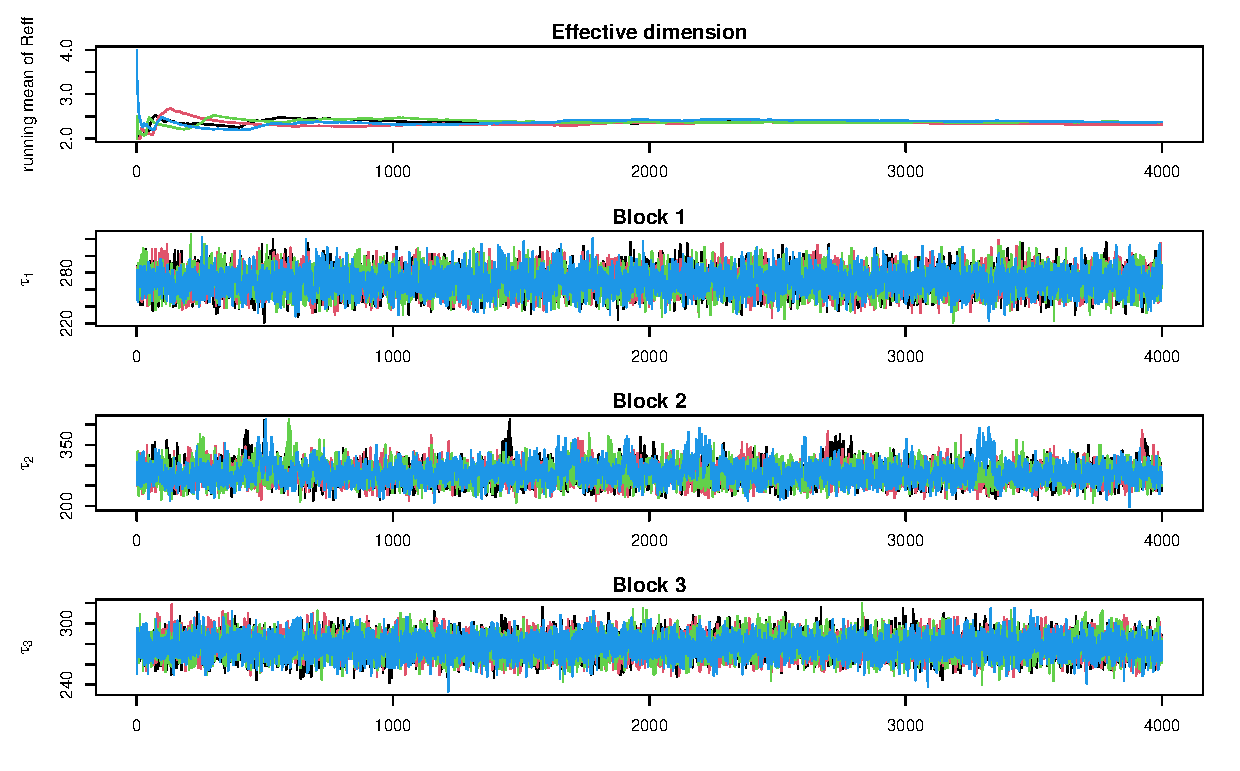
\includegraphics[width=\linewidth]{figs/diagnostic1.eps}
 \caption{MCMC diagnostics for $s=0.06$: running mean of $\Reff$ and traces of the noise precisions $\tau_k$ for the four chains.\label{fig:diag1}} 
\end{figure}

\begin{figure}
 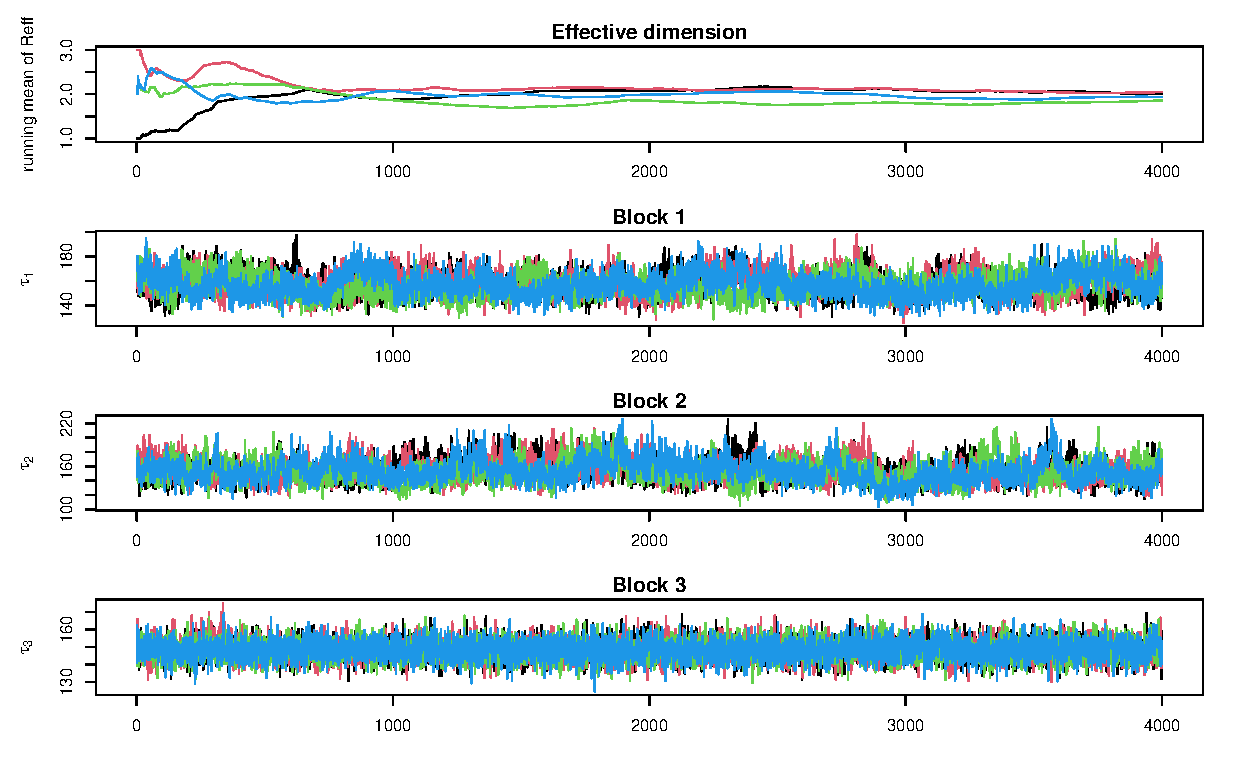
\includegraphics[width=\linewidth]{figs/diagnostic2.eps}
 \caption{MCMC diagnostics for $s=0.08$: running mean of $\Reff$ and traces of the noise precisions $\tau_k$ for the four chains.\label{fig:diag2}} 
\end{figure}

\section{Saturation of the effective rank on the breast cancer data}\label{sec:saturation}
 
Table~\ref{tab:saturation} reports short runs of the sparse Gibbs sampler ($R_{\max}=20$, $\lambda=1$, $a_\theta=b_\theta=1$) on three kinds of data with the dimensions of the breast cancer data ($N=150$, $p_k=184,200,142$), from the two initialisations of the indicators. \textcolor{red}{[Short runs of 800--1000 iterations (burn-in 400--500); to be rerun with the settings of the main analysis and several replications before publication.]}
 
\begin{table}[ht]
\centering
\begin{tabular}{lcccc}
  \hline
  & \multicolumn{2}{c}{$\gamma$ initialised to 1} & \multicolumn{2}{c}{$\gamma$ initialised to 0} \\
  Data & $\EE[\Reff\mid\X]$ & active per block & $\EE[\Reff\mid\X]$ & active per block \\
  \hline
  i.i.d.\ Gaussian noise & 0.7 & 0.3 / 0.1 / 0.2 & 1.3 & 0.4 / 0.6 / 0.5 \\
  heteroscedastic noise$^a$ & 20 & 6.0 / 4.8 / 15.2 & 12.5 & 3.3 / 2.6 / 8.4 \\
  TCGA, standardised & 20 & 17.1 / 15.0 / 15.9 & 15.1 & 11.7 / 9.9 / 11.8 \\
  \hline
\end{tabular}
\caption{Posterior mean of $\Reff$ and mean number of active dimensions in the miRNA / mRNA / protein blocks, for $R_{\max}=20$. $^a$Independent columns with the standard deviations of the TCGA variables and no common structure. \label{tab:saturation}}
\end{table}
 
\begin{figure}
 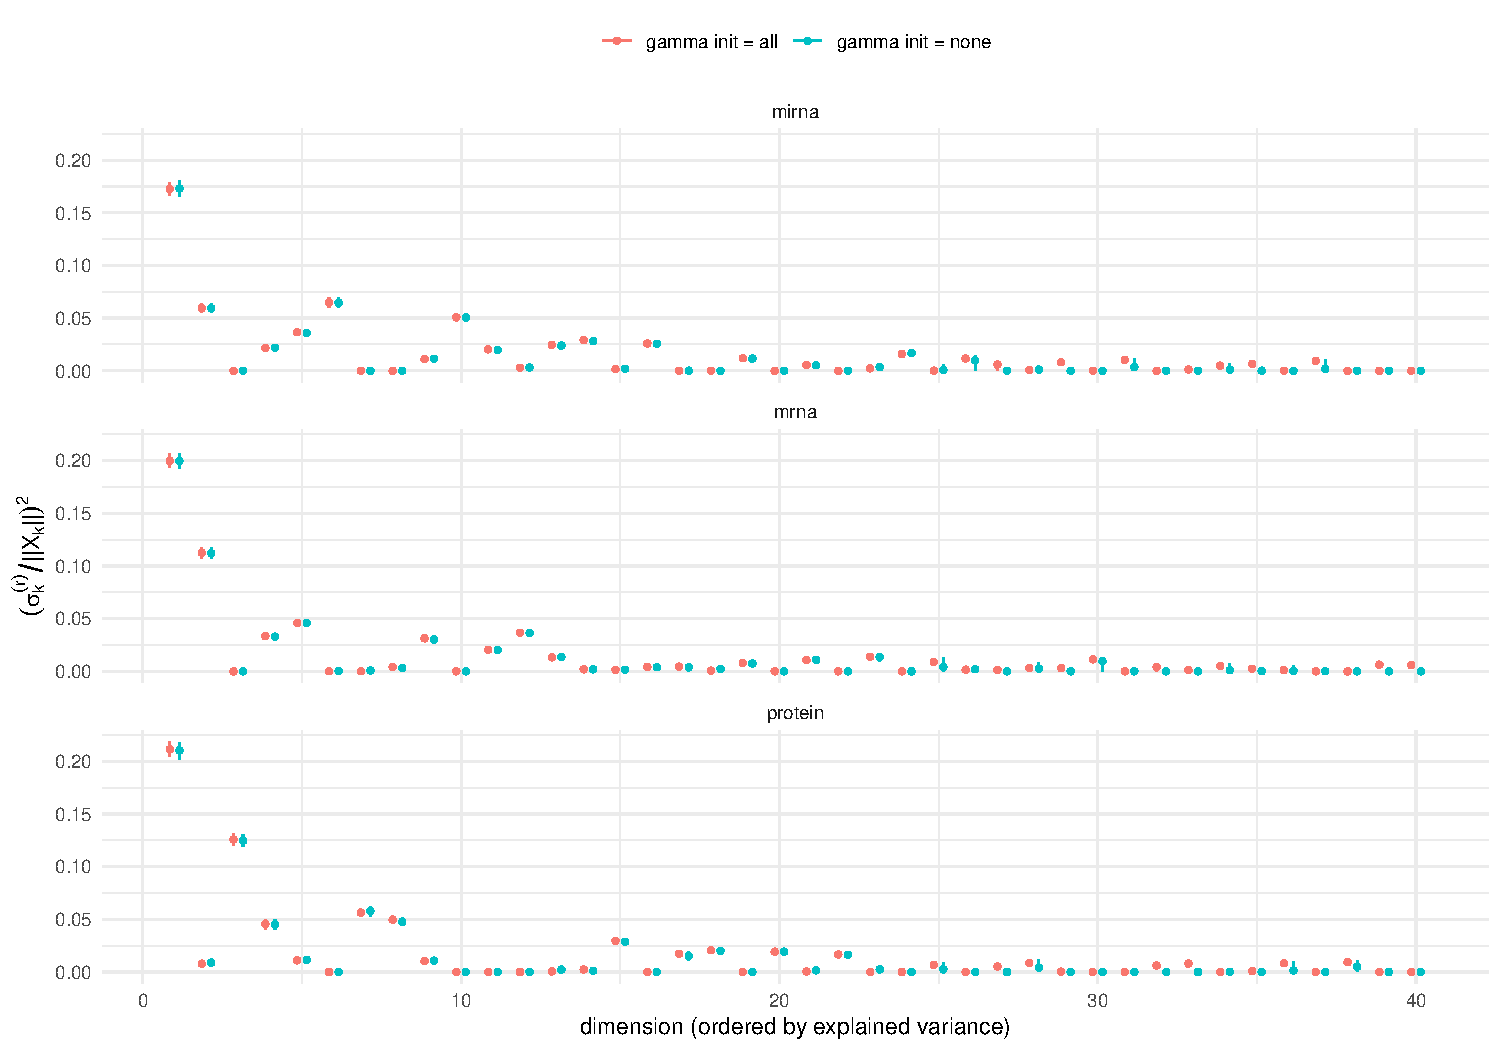
\includegraphics[width=\linewidth]{figs/weights_by_init.pdf}
 \caption{Breast cancer data: posterior means and 95\% credible intervals of the proportions of variance $(\sigma_k^{(r)}/\|\X_k\|)^2$, for the chains started with all the dimensions active and with none of them, the dimensions being ordered as in Figure~\ref{fig:tcga_weights}.}
\end{figure}
 
\begin{figure}
 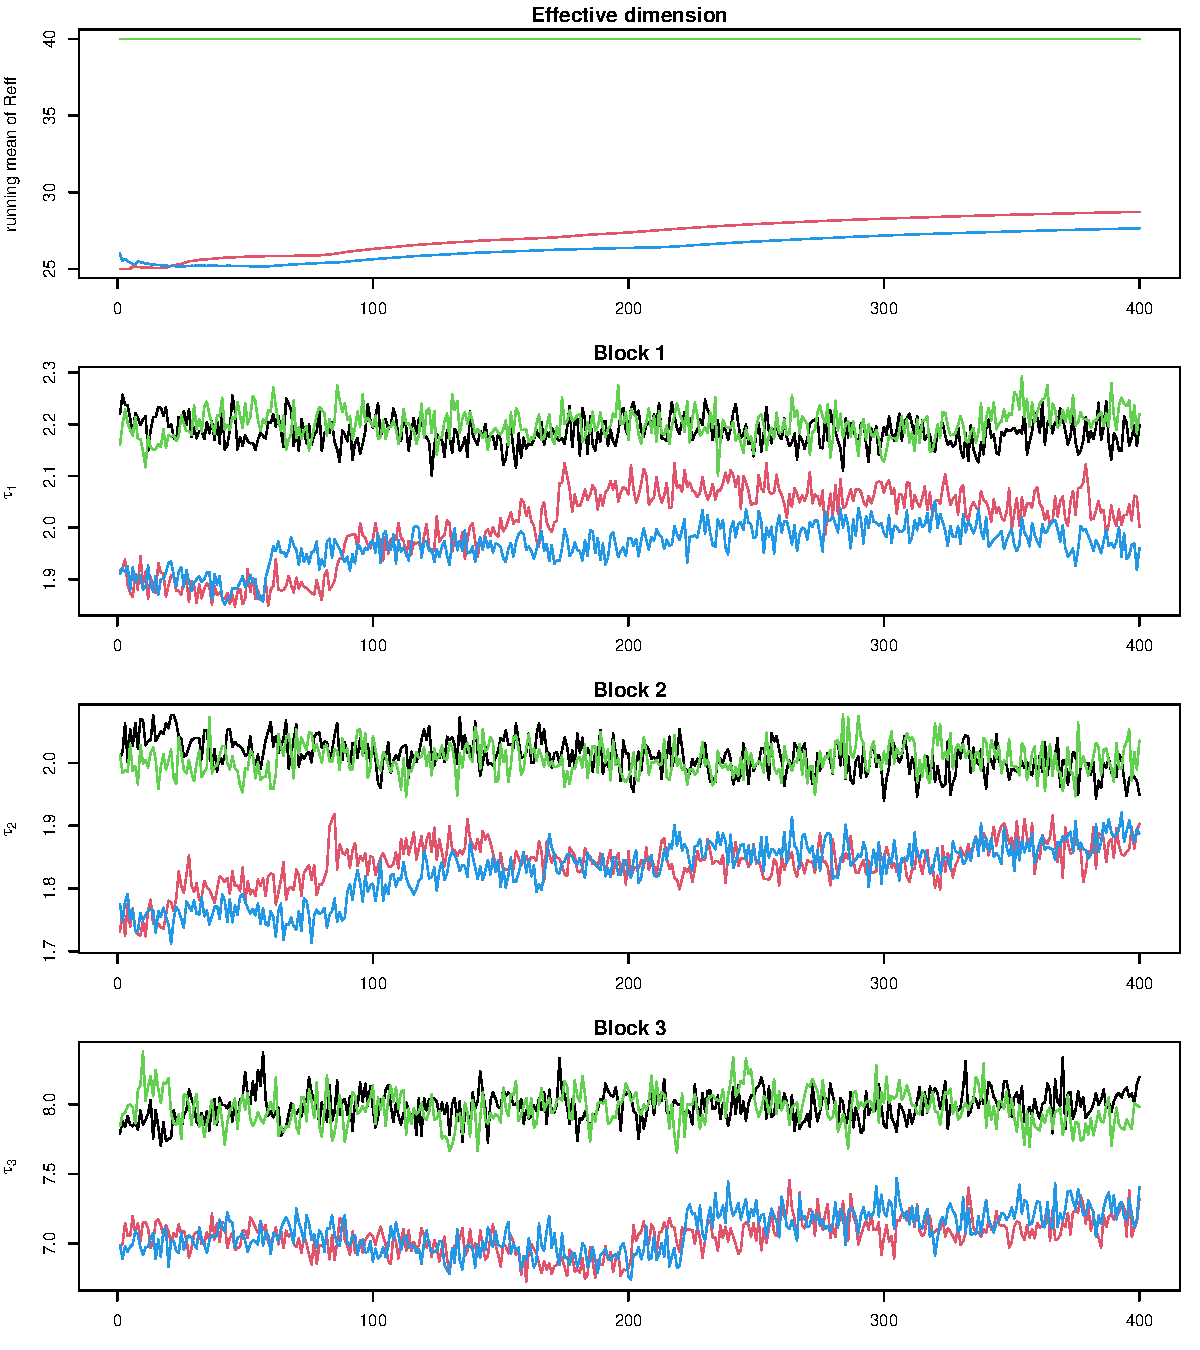
\includegraphics[width=\linewidth]{figs/diagnostics.pdf}
 \caption{Breast cancer data, MCMC diagnostics of the sparse Gibbs sampler ($R_{\max}=40$): running mean of $\Reff$ and traces of the noise precisions $\tau_k$ for the four chains (two started with $\gamma=1$, two with $\gamma=0$). \label{fig:tcga_diag}}
\end{figure}



\end{document}

